% --------------------------------------------------------------------------------
% ---------------------------------  Preamble  -----------------------------------
% --------------------------------------------------------------------------------

\documentclass{article}

\usepackage{microtype}

\usepackage[letterpaper, margin=0.75in]{geometry}
\usepackage{graphicx}               % to insert figures
\usepackage[table,x11names]{xcolor} % colors for e-copies
\usepackage{subcaption}             % subfigures
\usepackage{placeins}               % Float barriers
\usepackage{booktabs}
\usepackage{array}
\usepackage{caption}
\usepackage{rotating}
\usepackage{multicol}
\usepackage{multirow}
\usepackage{titlesec}
\usepackage{hyperref}               % PDF hyperreferences
\usepackage{titling}
\usepackage{tikz}
\usetikzlibrary{shapes.geometric}
\usetikzlibrary{calc}
\usepackage[T1]{fontenc}
\usepackage{ifthen}

\newcommand{\mysectiontitle}{}
\newcommand{\newsection}[2]{\renewcommand{\mysectiontitle}{#2}\section{#1}}

\newcommand{\Vline}[1]{}
\newcommand{\Hline}[1]{\hline}

\title{BattleTech: Outworlds Wastes}
\author{}
\date{}

\newcommand{\outworldsMode}{mode-web}

% --------------------------------------------------------------------------------
% ---------------------------------  Document  -----------------------------------
% --------------------------------------------------------------------------------

\begin{document}

\makeatletter
\Tag{TITLE+}{\@title}

\begin{center}
  \mbox{
\HCode{<div style="min-width: max-content; text-align: center">}
\fontsize{50}{60}\bfseries\selectfont{\MakeUppercase{B}}\includegraphics[alt='a', width=0.6in, height=0.6in]{img/Battletech-A.png}\fontsize{50}{60}\bfseries\selectfont{\MakeUppercase{ttleTech}}
\HCode{</div>}
}

  \fontsize{30}{37}\bfseries\selectfont\MakeUppercase{Outworlds Wastes}

  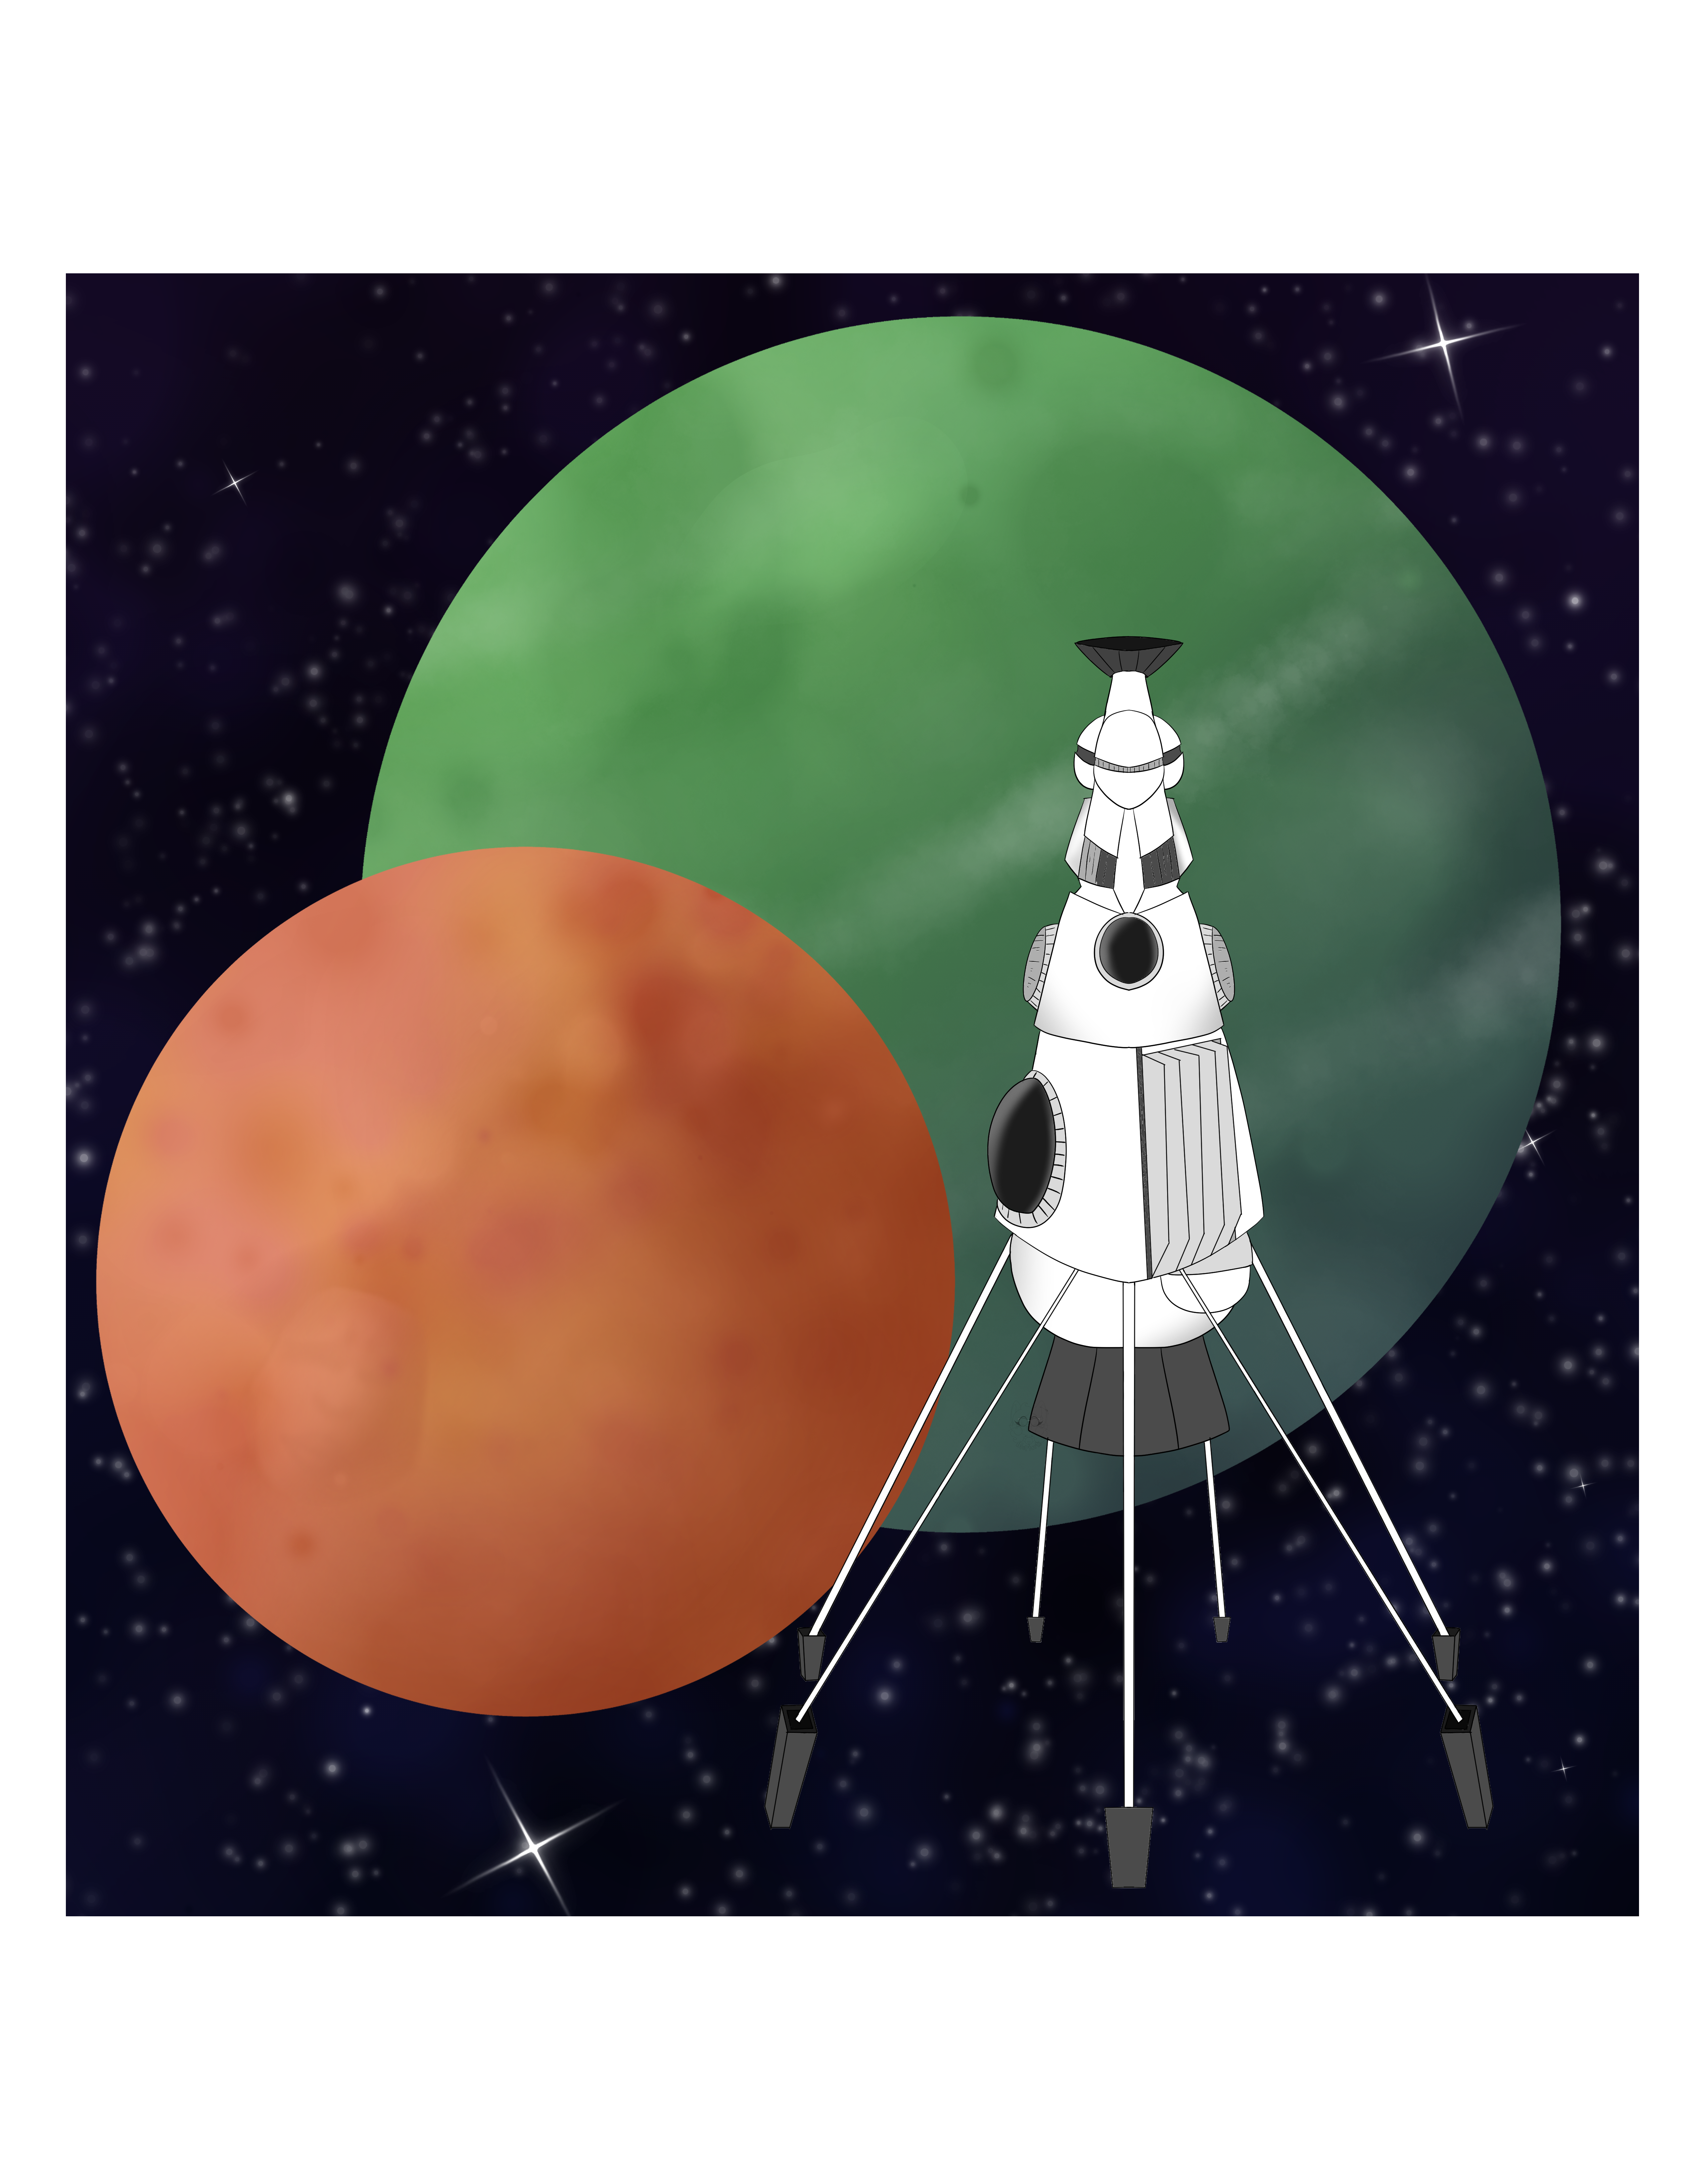
\includegraphics[alt='Outworlds Wastes logo', width=4.79in, height=5in]{img/Outworlds-Wastes.png}

  \LARGE\bfseries{Casual BattleTech Campaign League}
\end{center}

% --------------------------------------------------------------------------------
\newsection{Introduction}{introduction}
% --------------------------------------------------------------------------------

The event format provides faster, simplified rules which are more suitable for playing multiple scenarios in a large event, such as at a convention.


% --------------------------------------------------------------------------------
\subsection{Force Construction}
\label{subsec:force_construction}
% --------------------------------------------------------------------------------

Commanders create an initial force of up to 10,000 BV.
BV costs for all units are listed in the \href{http://www.masterunitlist.info}{Master Unit List} or \href{https://megamek.org}{MegaMekLab}.
Force construction must follow the following rules:

\begin{itemize}

\item Commanders have a modified Union class DropShip with 15 configurable bays.
Bays may be empty and can changed to a different configuration.
Bay space for all infantry units is shared across bays.
Your entire force must fit onto your DropShip.
Bay limits are in the table below.

\begin{table}[!h]
\ifthenelse{\not \equal{\outworldsMode}{mode-web}}{\fontfamily{Montserrat-LF}}{\small}\selectfont
\centering
\newcolumntype{R}[1]{>{\raggedleft\let\newline\\\arraybackslash\hspace{0pt}}m{#1}}
\begin{tabular}{!{\Vline{1pt}} m{10em} m{20em} R{3.8em} !{\Vline{1pt}}}
\Hline{1pt}
\rowcolor{black!30}  \bfseries{Bay Type} & \bfseries{Capacity} & \bfseries{Limit} \\
\Hline{1pt}
'Mech            & 1 'Mech or 1/2 superheavy 'Mech    & 12 bays \\
Combat Vehicle   & 2 vehicles or 1 superheavy vehicle & 5 bays  \\
Aerospace        & 1 aerospace unit                   & 2 bays  \\
ProtoMech        & 5 ProtoMechs                       & 2 bays  \\
Infantry         & 15 tons or 1 unit over 15 tons     & 2 bays  \\
\Hline{1pt}
\end{tabular}
\caption*{DropShip Bay Limits}
\end{table}

Support, Advanced Support, and Advanced Aerospace units are not permitted.
Illegal designs and units over 200 tons are also not permitted.
Units over 100 tons, such as superheavy 'Mechs, require double the bay space as standard units.

\item Commanders must select units from their faction on the \href{http://www.masterunitlist.info/}{Master Unit List} for the era chosen by league organizers.
Forces can include units with introductory, standard, or advanced technology.
For example, the Marauder MAD-3R is a valid ilClan era mercenary unit.

\item Forces may include one Unique or Experimental unit.
The Unique unit may be Extinct if another variant of the unit is available to the faction in the current era and the faction has the relevant technology base to recreate the unit.

\item Each force can start with no more than 7,000 BV in 'Mechs.
Commanders are encouraged to try to use the typical 'Mech unit composition of their faction.

\item Some scenarios will require infantry/Battle Armor or Combat Vehicles with cargo capacity, so commanders should have at least one of each of these units in their force.

\item Unless optional Battlefield Support or off-board artillery rules are used, a force can only include on-map units.
For example, artillery and aerospace units can only be used on-map by default.

\item The BV cost of a unit includes the skill level.
The initial skill levels for a unit may be no better than Gunnery 3/Piloting 4 and cannot differ by more than 3.
Average skill levels for factions and units are given on \emph{BattleTech: Total Warfare} p. 40.
ProtoMechs always have Piloting 5 and infantry units without anti-'Mech equipment have Anti-'Mech 5, because these skills are not used for these units.

\end{itemize}

Commanders are responsible for knowing which rulebooks contain the rules pertaining to all units and special equipment in their force.

Unit record sheets can be generated using \href{https://megamek.org}{MegaMekLab} or similar tools.
BV costs sometimes do not mach between the \href{http://www.masterunitlist.info}{Master Unit List} and \href{https://megamek.org}{MegaMekLab}, especially for infantry units.
Commanders must use the same source for all BV costs.
All record sheets must agree with the BV costs from this source.

Learning new types of units can be intimidating.
Commanders may limit the types of different units in their non-'Mech forces.
For example, a force could include only troop transports and Battle Armor so the commander can meet any objectives while keeping new rules to a minimum.


\newpage

% --------------------------------------------------------------------------------
\subsection{Sample Forces}
\label{subsec:sample_forces}
% --------------------------------------------------------------------------------

Two sample initial forces are provided below.
The first force is a Civil War era mercenary company and the second force is an ilClan era Raven Alliance Nova.
Pilot names are encouraged, as one of the goals of \emph{BattleTech: Outworlds Wastes} is to develop the personalized lore for your force.

\begin{table}[!h]
\ifthenelse{\not \equal{\outworldsMode}{mode-web}}{\fontfamily{Montserrat-LF}}{\small}\selectfont
\centering
\newcolumntype{R}[1]{>{\raggedleft\let\newline\\\arraybackslash\hspace{0pt}}m{#1}}
\begin{tabular}{!{\Vline{1pt}} m{2em} m{12em} m{8em} R{4.6em} R{4.6em} R{3.5em} R{3.8em} !{\Vline{1pt}}}
\Hline{1pt}
\rowcolor{black!30}  \bfseries{Bay} & \bfseries{Unit} & \bfseries{Pilot} & \bfseries{Gunnery} & \bfseries{Piloting} & \bfseries{BV} & \bfseries{Adj BV} \\
\Hline{1pt}
\rowcolor{black!30} \multicolumn{7}{!{\Vline{1pt}}c!{\Vline{1pt}}}{'Mechs} \\
\Hline{1pt}
1   & Atlas AS7-D           & 'Meg' Courant    & 3       & 4         & 1,897 & 2,504 \\
2   & Phoenix Hawk PXH-2K   & 'Bison' Helge    & 4       & 5         & 1,271 & 1,271 \\
3   & Blackjack BJ-2        & 'Lizard' Baker   & 4       & 5         & 1,148 & 1,148 \\
4   & Locust IIC            & 'Casper' Poole   & 4       & 5         & 1,100 & 1,100 \\
\Hline{1pt}
\rowcolor{black!30}\multicolumn{7}{!{\Vline{1pt}}c!{\Vline{1pt}}}{Combat Vehicles} \\
\Hline{1pt}
1  & Maxim Hover Transport &                   & 4       & 5         &   764 &   764 \\
1  & Maxim Hover Transport &                   & 4       & 5         &   764 &   764 \\
2  & Galleon GAL-102       &                   & 4       & 5         &   651 &   651 \\
2  & Galleon GAL-102       &                   & 4       & 5         &   651 &   651 \\
3  & Warrior H-7           &                   & 4       & 5         &   295 &   295 \\
3  & Warrior H-7           &                   & 4       & 5         &   295 &   295 \\
\Hline{1pt}
\rowcolor{black!30}\multicolumn{7}{!{\Vline{1pt}}c!{\Vline{1pt}}}{Infantry/Battle Armor} \\
\Hline{1pt}
1  & IS Std BA, LRR        &                   & 4       & 5         &   255 &   255 \\
1  & IS Std BA, Laser      &                   & 4       & 5         &   231 &   231 \\
\Hline{1pt}
8  & Total Bays            &                   &         &           &       &       \\
   & Total BV              &                   &         &           &       & 9,929 \\
\Hline{1pt}
\end{tabular}
\caption*{Civil War Era Mercenary Force - Meg's Magpies}
\end{table}

\begin{table}[!h]
\ifthenelse{\not \equal{\outworldsMode}{mode-web}}{\fontfamily{Montserrat-LF}}{\small}\selectfont
\centering
\newcolumntype{R}[1]{>{\raggedleft\let\newline\\\arraybackslash\hspace{0pt}}m{#1}}
\begin{tabular}{!{\Vline{1pt}} m{2em} m{12em} m{8em} R{4.6em} R{4.6em} R{3.5em} R{3.8em} !{\Vline{1pt}}}
\Hline{1pt}
\rowcolor{black!30}  \bfseries{Bay} & \bfseries{Unit} & \bfseries{Pilot} & \bfseries{Gunnery} & \bfseries{Piloting} & \bfseries{BV} & \bfseries{Adj BV} \\
\Hline{1pt}
\rowcolor{black!30}\multicolumn{7}{!{\Vline{1pt}}c!{\Vline{1pt}}}{'Mechs} \\
\Hline{1pt}
1 & Carrion Crow A        & Sarah Magnus    & 3       & 4         & 1,622 & 2,141 \\
2 & Nova U                &       Bryn      & 4       & 5         & 1,413 & 1,413 \\
3 & Adder J               &       Ada       & 4       & 5         & 1,222 & 1,222 \\
4 & Kit Fox V             &       Soton     & 3       & 4         &   974 & 1,286 \\
5 & Fire Moth A           &       Tina      & 3       & 4         &   639 &   843 \\
\Hline{1pt}
\rowcolor{black!30}\multicolumn{7}{!{\Vline{1pt}}c!{\Vline{1pt}}}{Combat Vehicles} \\
\Hline{1pt}
1 & Karnov UR Transport   &                 & 4       & 5          &   125 &   125 \\
\Hline{1pt}
\rowcolor{black!30}\multicolumn{7}{!{\Vline{1pt}}c!{\Vline{1pt}}}{Infantry/Battle Armor} \\
\Hline{1pt}
1 & Elemental BA, Laser   &                 & 3       & 4         &   447 &   590 \\
1 & Elemental BA, HMG     &                 & 3       & 4         &   415 &   548 \\
1 & Elemental BA, Flamer  &                 & 3       & 4         &   404 &   533 \\
2 & Elemental BA, Flamer  &                 & 3       & 4         &   404 &   533 \\
2 & Gnome BA              &                 & 3       & 4         &   580 &   766 \\
\Hline{1pt}
8 & Total Bays            &                 &         &           &       &       \\
  & Total BV              &                 &         &           &       & 10,000 \\
\Hline{1pt}
\end{tabular}
\caption*{ilClan Era Raven Alliance Force - Raven Expeditionary Cluster, Alpha Nova}
\end{table}

Both forces can support additional units on their DropShips.
However, the Raven Alliance force cannot add any additional infantry bays because the DropShip has the maximum of 5 infantry bays.


\newpage

% --------------------------------------------------------------------------------
\subsection{Advanced Force Construction Rules}
% --------------------------------------------------------------------------------

\input{2-Force-Construction/2-Advanced-Force-Construction.tex}

\begin{figure}[!h]
  \begin{center}
  \begin{subfigure}{0.4\textwidth}
    \centering
    \frame{\includegraphics[alt='Clan Dark Caste Faction list', height=4.9in, width=2.4in]{img/Dark-Caste-List.png}}
    \caption*{Clan Dark Caste\\Civil War Era}
  \end{subfigure}
  \hspace{1in}
  \begin{subfigure}{0.4\textwidth}
    \centering
    \frame{\includegraphics[alt='Combine Mercenary Faction list', height=4.9in, width=2.4in]{img/Combine-Mercenary-List.png}}
    \caption*{Combine Mercenary\\Clan Invasion Era}
  \end{subfigure}
  \ifthenelse{\equal{\outworldsMode}{mode-pdf}}{\caption*{Custom Faction Lists}}{}
  \end{center}
\end{figure}


\newpage


\newpage

% --------------------------------------------------------------------------------
\newsection{Background}{background}
% --------------------------------------------------------------------------------

The event format provides faster, simplified rules which are more suitable for playing multiple scenarios in a large event, such as at a convention.


% --------------------------------------------------------------------------------
\subsection{Force Construction}
\label{subsec:force_construction}
% --------------------------------------------------------------------------------

Commanders create an initial force of up to 10,000 BV.
BV costs for all units are listed in the \href{http://www.masterunitlist.info}{Master Unit List} or \href{https://megamek.org}{MegaMekLab}.
Force construction must follow the following rules:

\begin{itemize}

\item Commanders have a modified Union class DropShip with 15 configurable bays.
Bays may be empty and can changed to a different configuration.
Bay space for all infantry units is shared across bays.
Your entire force must fit onto your DropShip.
Bay limits are in the table below.

\begin{table}[!h]
\ifthenelse{\not \equal{\outworldsMode}{mode-web}}{\fontfamily{Montserrat-LF}}{\small}\selectfont
\centering
\newcolumntype{R}[1]{>{\raggedleft\let\newline\\\arraybackslash\hspace{0pt}}m{#1}}
\begin{tabular}{!{\Vline{1pt}} m{10em} m{20em} R{3.8em} !{\Vline{1pt}}}
\Hline{1pt}
\rowcolor{black!30}  \bfseries{Bay Type} & \bfseries{Capacity} & \bfseries{Limit} \\
\Hline{1pt}
'Mech            & 1 'Mech or 1/2 superheavy 'Mech    & 12 bays \\
Combat Vehicle   & 2 vehicles or 1 superheavy vehicle & 5 bays  \\
Aerospace        & 1 aerospace unit                   & 2 bays  \\
ProtoMech        & 5 ProtoMechs                       & 2 bays  \\
Infantry         & 15 tons or 1 unit over 15 tons     & 2 bays  \\
\Hline{1pt}
\end{tabular}
\caption*{DropShip Bay Limits}
\end{table}

Support, Advanced Support, and Advanced Aerospace units are not permitted.
Illegal designs and units over 200 tons are also not permitted.
Units over 100 tons, such as superheavy 'Mechs, require double the bay space as standard units.

\item Commanders must select units from their faction on the \href{http://www.masterunitlist.info/}{Master Unit List} for the era chosen by league organizers.
Forces can include units with introductory, standard, or advanced technology.
For example, the Marauder MAD-3R is a valid ilClan era mercenary unit.

\item Forces may include one Unique or Experimental unit.
The Unique unit may be Extinct if another variant of the unit is available to the faction in the current era and the faction has the relevant technology base to recreate the unit.

\item Each force can start with no more than 7,000 BV in 'Mechs.
Commanders are encouraged to try to use the typical 'Mech unit composition of their faction.

\item Some scenarios will require infantry/Battle Armor or Combat Vehicles with cargo capacity, so commanders should have at least one of each of these units in their force.

\item Unless optional Battlefield Support or off-board artillery rules are used, a force can only include on-map units.
For example, artillery and aerospace units can only be used on-map by default.

\item The BV cost of a unit includes the skill level.
The initial skill levels for a unit may be no better than Gunnery 3/Piloting 4 and cannot differ by more than 3.
Average skill levels for factions and units are given on \emph{BattleTech: Total Warfare} p. 40.
ProtoMechs always have Piloting 5 and infantry units without anti-'Mech equipment have Anti-'Mech 5, because these skills are not used for these units.

\end{itemize}

Commanders are responsible for knowing which rulebooks contain the rules pertaining to all units and special equipment in their force.

Unit record sheets can be generated using \href{https://megamek.org}{MegaMekLab} or similar tools.
BV costs sometimes do not mach between the \href{http://www.masterunitlist.info}{Master Unit List} and \href{https://megamek.org}{MegaMekLab}, especially for infantry units.
Commanders must use the same source for all BV costs.
All record sheets must agree with the BV costs from this source.

Learning new types of units can be intimidating.
Commanders may limit the types of different units in their non-'Mech forces.
For example, a force could include only troop transports and Battle Armor so the commander can meet any objectives while keeping new rules to a minimum.


\newpage

% --------------------------------------------------------------------------------
\subsection{Sample Forces}
\label{subsec:sample_forces}
% --------------------------------------------------------------------------------

Two sample initial forces are provided below.
The first force is a Civil War era mercenary company and the second force is an ilClan era Raven Alliance Nova.
Pilot names are encouraged, as one of the goals of \emph{BattleTech: Outworlds Wastes} is to develop the personalized lore for your force.

\begin{table}[!h]
\ifthenelse{\not \equal{\outworldsMode}{mode-web}}{\fontfamily{Montserrat-LF}}{\small}\selectfont
\centering
\newcolumntype{R}[1]{>{\raggedleft\let\newline\\\arraybackslash\hspace{0pt}}m{#1}}
\begin{tabular}{!{\Vline{1pt}} m{2em} m{12em} m{8em} R{4.6em} R{4.6em} R{3.5em} R{3.8em} !{\Vline{1pt}}}
\Hline{1pt}
\rowcolor{black!30}  \bfseries{Bay} & \bfseries{Unit} & \bfseries{Pilot} & \bfseries{Gunnery} & \bfseries{Piloting} & \bfseries{BV} & \bfseries{Adj BV} \\
\Hline{1pt}
\rowcolor{black!30} \multicolumn{7}{!{\Vline{1pt}}c!{\Vline{1pt}}}{'Mechs} \\
\Hline{1pt}
1   & Atlas AS7-D           & 'Meg' Courant    & 3       & 4         & 1,897 & 2,504 \\
2   & Phoenix Hawk PXH-2K   & 'Bison' Helge    & 4       & 5         & 1,271 & 1,271 \\
3   & Blackjack BJ-2        & 'Lizard' Baker   & 4       & 5         & 1,148 & 1,148 \\
4   & Locust IIC            & 'Casper' Poole   & 4       & 5         & 1,100 & 1,100 \\
\Hline{1pt}
\rowcolor{black!30}\multicolumn{7}{!{\Vline{1pt}}c!{\Vline{1pt}}}{Combat Vehicles} \\
\Hline{1pt}
1  & Maxim Hover Transport &                   & 4       & 5         &   764 &   764 \\
1  & Maxim Hover Transport &                   & 4       & 5         &   764 &   764 \\
2  & Galleon GAL-102       &                   & 4       & 5         &   651 &   651 \\
2  & Galleon GAL-102       &                   & 4       & 5         &   651 &   651 \\
3  & Warrior H-7           &                   & 4       & 5         &   295 &   295 \\
3  & Warrior H-7           &                   & 4       & 5         &   295 &   295 \\
\Hline{1pt}
\rowcolor{black!30}\multicolumn{7}{!{\Vline{1pt}}c!{\Vline{1pt}}}{Infantry/Battle Armor} \\
\Hline{1pt}
1  & IS Std BA, LRR        &                   & 4       & 5         &   255 &   255 \\
1  & IS Std BA, Laser      &                   & 4       & 5         &   231 &   231 \\
\Hline{1pt}
8  & Total Bays            &                   &         &           &       &       \\
   & Total BV              &                   &         &           &       & 9,929 \\
\Hline{1pt}
\end{tabular}
\caption*{Civil War Era Mercenary Force - Meg's Magpies}
\end{table}

\begin{table}[!h]
\ifthenelse{\not \equal{\outworldsMode}{mode-web}}{\fontfamily{Montserrat-LF}}{\small}\selectfont
\centering
\newcolumntype{R}[1]{>{\raggedleft\let\newline\\\arraybackslash\hspace{0pt}}m{#1}}
\begin{tabular}{!{\Vline{1pt}} m{2em} m{12em} m{8em} R{4.6em} R{4.6em} R{3.5em} R{3.8em} !{\Vline{1pt}}}
\Hline{1pt}
\rowcolor{black!30}  \bfseries{Bay} & \bfseries{Unit} & \bfseries{Pilot} & \bfseries{Gunnery} & \bfseries{Piloting} & \bfseries{BV} & \bfseries{Adj BV} \\
\Hline{1pt}
\rowcolor{black!30}\multicolumn{7}{!{\Vline{1pt}}c!{\Vline{1pt}}}{'Mechs} \\
\Hline{1pt}
1 & Carrion Crow A        & Sarah Magnus    & 3       & 4         & 1,622 & 2,141 \\
2 & Nova U                &       Bryn      & 4       & 5         & 1,413 & 1,413 \\
3 & Adder J               &       Ada       & 4       & 5         & 1,222 & 1,222 \\
4 & Kit Fox V             &       Soton     & 3       & 4         &   974 & 1,286 \\
5 & Fire Moth A           &       Tina      & 3       & 4         &   639 &   843 \\
\Hline{1pt}
\rowcolor{black!30}\multicolumn{7}{!{\Vline{1pt}}c!{\Vline{1pt}}}{Combat Vehicles} \\
\Hline{1pt}
1 & Karnov UR Transport   &                 & 4       & 5          &   125 &   125 \\
\Hline{1pt}
\rowcolor{black!30}\multicolumn{7}{!{\Vline{1pt}}c!{\Vline{1pt}}}{Infantry/Battle Armor} \\
\Hline{1pt}
1 & Elemental BA, Laser   &                 & 3       & 4         &   447 &   590 \\
1 & Elemental BA, HMG     &                 & 3       & 4         &   415 &   548 \\
1 & Elemental BA, Flamer  &                 & 3       & 4         &   404 &   533 \\
2 & Elemental BA, Flamer  &                 & 3       & 4         &   404 &   533 \\
2 & Gnome BA              &                 & 3       & 4         &   580 &   766 \\
\Hline{1pt}
8 & Total Bays            &                 &         &           &       &       \\
  & Total BV              &                 &         &           &       & 10,000 \\
\Hline{1pt}
\end{tabular}
\caption*{ilClan Era Raven Alliance Force - Raven Expeditionary Cluster, Alpha Nova}
\end{table}

Both forces can support additional units on their DropShips.
However, the Raven Alliance force cannot add any additional infantry bays because the DropShip has the maximum of 5 infantry bays.


\newpage

% --------------------------------------------------------------------------------
\subsection{Advanced Force Construction Rules}
% --------------------------------------------------------------------------------

\input{2-Force-Construction/2-Advanced-Force-Construction.tex}

\begin{figure}[!h]
  \begin{center}
  \begin{subfigure}{0.4\textwidth}
    \centering
    \frame{\includegraphics[alt='Clan Dark Caste Faction list', height=4.9in, width=2.4in]{img/Dark-Caste-List.png}}
    \caption*{Clan Dark Caste\\Civil War Era}
  \end{subfigure}
  \hspace{1in}
  \begin{subfigure}{0.4\textwidth}
    \centering
    \frame{\includegraphics[alt='Combine Mercenary Faction list', height=4.9in, width=2.4in]{img/Combine-Mercenary-List.png}}
    \caption*{Combine Mercenary\\Clan Invasion Era}
  \end{subfigure}
  \ifthenelse{\equal{\outworldsMode}{mode-pdf}}{\caption*{Custom Faction Lists}}{}
  \end{center}
\end{figure}


\newpage


% --------------------------------------------------------------------------------
\newsection{Force Construction}{force-construction}
% --------------------------------------------------------------------------------

The event format provides faster, simplified rules which are more suitable for playing multiple scenarios in a large event, such as at a convention.


% --------------------------------------------------------------------------------
\subsection{Force Construction}
\label{subsec:force_construction}
% --------------------------------------------------------------------------------

Commanders create an initial force of up to 10,000 BV.
BV costs for all units are listed in the \href{http://www.masterunitlist.info}{Master Unit List} or \href{https://megamek.org}{MegaMekLab}.
Force construction must follow the following rules:

\begin{itemize}

\item Commanders have a modified Union class DropShip with 15 configurable bays.
Bays may be empty and can changed to a different configuration.
Bay space for all infantry units is shared across bays.
Your entire force must fit onto your DropShip.
Bay limits are in the table below.

\begin{table}[!h]
\ifthenelse{\not \equal{\outworldsMode}{mode-web}}{\fontfamily{Montserrat-LF}}{\small}\selectfont
\centering
\newcolumntype{R}[1]{>{\raggedleft\let\newline\\\arraybackslash\hspace{0pt}}m{#1}}
\begin{tabular}{!{\Vline{1pt}} m{10em} m{20em} R{3.8em} !{\Vline{1pt}}}
\Hline{1pt}
\rowcolor{black!30}  \bfseries{Bay Type} & \bfseries{Capacity} & \bfseries{Limit} \\
\Hline{1pt}
'Mech            & 1 'Mech or 1/2 superheavy 'Mech    & 12 bays \\
Combat Vehicle   & 2 vehicles or 1 superheavy vehicle & 5 bays  \\
Aerospace        & 1 aerospace unit                   & 2 bays  \\
ProtoMech        & 5 ProtoMechs                       & 2 bays  \\
Infantry         & 15 tons or 1 unit over 15 tons     & 2 bays  \\
\Hline{1pt}
\end{tabular}
\caption*{DropShip Bay Limits}
\end{table}

Support, Advanced Support, and Advanced Aerospace units are not permitted.
Illegal designs and units over 200 tons are also not permitted.
Units over 100 tons, such as superheavy 'Mechs, require double the bay space as standard units.

\item Commanders must select units from their faction on the \href{http://www.masterunitlist.info/}{Master Unit List} for the era chosen by league organizers.
Forces can include units with introductory, standard, or advanced technology.
For example, the Marauder MAD-3R is a valid ilClan era mercenary unit.

\item Forces may include one Unique or Experimental unit.
The Unique unit may be Extinct if another variant of the unit is available to the faction in the current era and the faction has the relevant technology base to recreate the unit.

\item Each force can start with no more than 7,000 BV in 'Mechs.
Commanders are encouraged to try to use the typical 'Mech unit composition of their faction.

\item Some scenarios will require infantry/Battle Armor or Combat Vehicles with cargo capacity, so commanders should have at least one of each of these units in their force.

\item Unless optional Battlefield Support or off-board artillery rules are used, a force can only include on-map units.
For example, artillery and aerospace units can only be used on-map by default.

\item The BV cost of a unit includes the skill level.
The initial skill levels for a unit may be no better than Gunnery 3/Piloting 4 and cannot differ by more than 3.
Average skill levels for factions and units are given on \emph{BattleTech: Total Warfare} p. 40.
ProtoMechs always have Piloting 5 and infantry units without anti-'Mech equipment have Anti-'Mech 5, because these skills are not used for these units.

\end{itemize}

Commanders are responsible for knowing which rulebooks contain the rules pertaining to all units and special equipment in their force.

Unit record sheets can be generated using \href{https://megamek.org}{MegaMekLab} or similar tools.
BV costs sometimes do not mach between the \href{http://www.masterunitlist.info}{Master Unit List} and \href{https://megamek.org}{MegaMekLab}, especially for infantry units.
Commanders must use the same source for all BV costs.
All record sheets must agree with the BV costs from this source.

Learning new types of units can be intimidating.
Commanders may limit the types of different units in their non-'Mech forces.
For example, a force could include only troop transports and Battle Armor so the commander can meet any objectives while keeping new rules to a minimum.


\newpage

% --------------------------------------------------------------------------------
\subsection{Sample Forces}
\label{subsec:sample_forces}
% --------------------------------------------------------------------------------

Two sample initial forces are provided below.
The first force is a Civil War era mercenary company and the second force is an ilClan era Raven Alliance Nova.
Pilot names are encouraged, as one of the goals of \emph{BattleTech: Outworlds Wastes} is to develop the personalized lore for your force.

\begin{table}[!h]
\ifthenelse{\not \equal{\outworldsMode}{mode-web}}{\fontfamily{Montserrat-LF}}{\small}\selectfont
\centering
\newcolumntype{R}[1]{>{\raggedleft\let\newline\\\arraybackslash\hspace{0pt}}m{#1}}
\begin{tabular}{!{\Vline{1pt}} m{2em} m{12em} m{8em} R{4.6em} R{4.6em} R{3.5em} R{3.8em} !{\Vline{1pt}}}
\Hline{1pt}
\rowcolor{black!30}  \bfseries{Bay} & \bfseries{Unit} & \bfseries{Pilot} & \bfseries{Gunnery} & \bfseries{Piloting} & \bfseries{BV} & \bfseries{Adj BV} \\
\Hline{1pt}
\rowcolor{black!30} \multicolumn{7}{!{\Vline{1pt}}c!{\Vline{1pt}}}{'Mechs} \\
\Hline{1pt}
1   & Atlas AS7-D           & 'Meg' Courant    & 3       & 4         & 1,897 & 2,504 \\
2   & Phoenix Hawk PXH-2K   & 'Bison' Helge    & 4       & 5         & 1,271 & 1,271 \\
3   & Blackjack BJ-2        & 'Lizard' Baker   & 4       & 5         & 1,148 & 1,148 \\
4   & Locust IIC            & 'Casper' Poole   & 4       & 5         & 1,100 & 1,100 \\
\Hline{1pt}
\rowcolor{black!30}\multicolumn{7}{!{\Vline{1pt}}c!{\Vline{1pt}}}{Combat Vehicles} \\
\Hline{1pt}
1  & Maxim Hover Transport &                   & 4       & 5         &   764 &   764 \\
1  & Maxim Hover Transport &                   & 4       & 5         &   764 &   764 \\
2  & Galleon GAL-102       &                   & 4       & 5         &   651 &   651 \\
2  & Galleon GAL-102       &                   & 4       & 5         &   651 &   651 \\
3  & Warrior H-7           &                   & 4       & 5         &   295 &   295 \\
3  & Warrior H-7           &                   & 4       & 5         &   295 &   295 \\
\Hline{1pt}
\rowcolor{black!30}\multicolumn{7}{!{\Vline{1pt}}c!{\Vline{1pt}}}{Infantry/Battle Armor} \\
\Hline{1pt}
1  & IS Std BA, LRR        &                   & 4       & 5         &   255 &   255 \\
1  & IS Std BA, Laser      &                   & 4       & 5         &   231 &   231 \\
\Hline{1pt}
8  & Total Bays            &                   &         &           &       &       \\
   & Total BV              &                   &         &           &       & 9,929 \\
\Hline{1pt}
\end{tabular}
\caption*{Civil War Era Mercenary Force - Meg's Magpies}
\end{table}

\begin{table}[!h]
\ifthenelse{\not \equal{\outworldsMode}{mode-web}}{\fontfamily{Montserrat-LF}}{\small}\selectfont
\centering
\newcolumntype{R}[1]{>{\raggedleft\let\newline\\\arraybackslash\hspace{0pt}}m{#1}}
\begin{tabular}{!{\Vline{1pt}} m{2em} m{12em} m{8em} R{4.6em} R{4.6em} R{3.5em} R{3.8em} !{\Vline{1pt}}}
\Hline{1pt}
\rowcolor{black!30}  \bfseries{Bay} & \bfseries{Unit} & \bfseries{Pilot} & \bfseries{Gunnery} & \bfseries{Piloting} & \bfseries{BV} & \bfseries{Adj BV} \\
\Hline{1pt}
\rowcolor{black!30}\multicolumn{7}{!{\Vline{1pt}}c!{\Vline{1pt}}}{'Mechs} \\
\Hline{1pt}
1 & Carrion Crow A        & Sarah Magnus    & 3       & 4         & 1,622 & 2,141 \\
2 & Nova U                &       Bryn      & 4       & 5         & 1,413 & 1,413 \\
3 & Adder J               &       Ada       & 4       & 5         & 1,222 & 1,222 \\
4 & Kit Fox V             &       Soton     & 3       & 4         &   974 & 1,286 \\
5 & Fire Moth A           &       Tina      & 3       & 4         &   639 &   843 \\
\Hline{1pt}
\rowcolor{black!30}\multicolumn{7}{!{\Vline{1pt}}c!{\Vline{1pt}}}{Combat Vehicles} \\
\Hline{1pt}
1 & Karnov UR Transport   &                 & 4       & 5          &   125 &   125 \\
\Hline{1pt}
\rowcolor{black!30}\multicolumn{7}{!{\Vline{1pt}}c!{\Vline{1pt}}}{Infantry/Battle Armor} \\
\Hline{1pt}
1 & Elemental BA, Laser   &                 & 3       & 4         &   447 &   590 \\
1 & Elemental BA, HMG     &                 & 3       & 4         &   415 &   548 \\
1 & Elemental BA, Flamer  &                 & 3       & 4         &   404 &   533 \\
2 & Elemental BA, Flamer  &                 & 3       & 4         &   404 &   533 \\
2 & Gnome BA              &                 & 3       & 4         &   580 &   766 \\
\Hline{1pt}
8 & Total Bays            &                 &         &           &       &       \\
  & Total BV              &                 &         &           &       & 10,000 \\
\Hline{1pt}
\end{tabular}
\caption*{ilClan Era Raven Alliance Force - Raven Expeditionary Cluster, Alpha Nova}
\end{table}

Both forces can support additional units on their DropShips.
However, the Raven Alliance force cannot add any additional infantry bays because the DropShip has the maximum of 5 infantry bays.


\newpage

% --------------------------------------------------------------------------------
\subsection{Advanced Force Construction Rules}
% --------------------------------------------------------------------------------

\input{2-Force-Construction/2-Advanced-Force-Construction.tex}

\begin{figure}[!h]
  \begin{center}
  \begin{subfigure}{0.4\textwidth}
    \centering
    \frame{\includegraphics[alt='Clan Dark Caste Faction list', height=4.9in, width=2.4in]{img/Dark-Caste-List.png}}
    \caption*{Clan Dark Caste\\Civil War Era}
  \end{subfigure}
  \hspace{1in}
  \begin{subfigure}{0.4\textwidth}
    \centering
    \frame{\includegraphics[alt='Combine Mercenary Faction list', height=4.9in, width=2.4in]{img/Combine-Mercenary-List.png}}
    \caption*{Combine Mercenary\\Clan Invasion Era}
  \end{subfigure}
  \ifthenelse{\equal{\outworldsMode}{mode-pdf}}{\caption*{Custom Faction Lists}}{}
  \end{center}
\end{figure}


\newpage


\newpage

% --------------------------------------------------------------------------------
\newsection{Force Management}{force-management}
% --------------------------------------------------------------------------------

The event format provides faster, simplified rules which are more suitable for playing multiple scenarios in a large event, such as at a convention.


% --------------------------------------------------------------------------------
\subsection{Force Construction}
\label{subsec:force_construction}
% --------------------------------------------------------------------------------

Commanders create an initial force of up to 10,000 BV.
BV costs for all units are listed in the \href{http://www.masterunitlist.info}{Master Unit List} or \href{https://megamek.org}{MegaMekLab}.
Force construction must follow the following rules:

\begin{itemize}

\item Commanders have a modified Union class DropShip with 15 configurable bays.
Bays may be empty and can changed to a different configuration.
Bay space for all infantry units is shared across bays.
Your entire force must fit onto your DropShip.
Bay limits are in the table below.

\begin{table}[!h]
\ifthenelse{\not \equal{\outworldsMode}{mode-web}}{\fontfamily{Montserrat-LF}}{\small}\selectfont
\centering
\newcolumntype{R}[1]{>{\raggedleft\let\newline\\\arraybackslash\hspace{0pt}}m{#1}}
\begin{tabular}{!{\Vline{1pt}} m{10em} m{20em} R{3.8em} !{\Vline{1pt}}}
\Hline{1pt}
\rowcolor{black!30}  \bfseries{Bay Type} & \bfseries{Capacity} & \bfseries{Limit} \\
\Hline{1pt}
'Mech            & 1 'Mech or 1/2 superheavy 'Mech    & 12 bays \\
Combat Vehicle   & 2 vehicles or 1 superheavy vehicle & 5 bays  \\
Aerospace        & 1 aerospace unit                   & 2 bays  \\
ProtoMech        & 5 ProtoMechs                       & 2 bays  \\
Infantry         & 15 tons or 1 unit over 15 tons     & 2 bays  \\
\Hline{1pt}
\end{tabular}
\caption*{DropShip Bay Limits}
\end{table}

Support, Advanced Support, and Advanced Aerospace units are not permitted.
Illegal designs and units over 200 tons are also not permitted.
Units over 100 tons, such as superheavy 'Mechs, require double the bay space as standard units.

\item Commanders must select units from their faction on the \href{http://www.masterunitlist.info/}{Master Unit List} for the era chosen by league organizers.
Forces can include units with introductory, standard, or advanced technology.
For example, the Marauder MAD-3R is a valid ilClan era mercenary unit.

\item Forces may include one Unique or Experimental unit.
The Unique unit may be Extinct if another variant of the unit is available to the faction in the current era and the faction has the relevant technology base to recreate the unit.

\item Each force can start with no more than 7,000 BV in 'Mechs.
Commanders are encouraged to try to use the typical 'Mech unit composition of their faction.

\item Some scenarios will require infantry/Battle Armor or Combat Vehicles with cargo capacity, so commanders should have at least one of each of these units in their force.

\item Unless optional Battlefield Support or off-board artillery rules are used, a force can only include on-map units.
For example, artillery and aerospace units can only be used on-map by default.

\item The BV cost of a unit includes the skill level.
The initial skill levels for a unit may be no better than Gunnery 3/Piloting 4 and cannot differ by more than 3.
Average skill levels for factions and units are given on \emph{BattleTech: Total Warfare} p. 40.
ProtoMechs always have Piloting 5 and infantry units without anti-'Mech equipment have Anti-'Mech 5, because these skills are not used for these units.

\end{itemize}

Commanders are responsible for knowing which rulebooks contain the rules pertaining to all units and special equipment in their force.

Unit record sheets can be generated using \href{https://megamek.org}{MegaMekLab} or similar tools.
BV costs sometimes do not mach between the \href{http://www.masterunitlist.info}{Master Unit List} and \href{https://megamek.org}{MegaMekLab}, especially for infantry units.
Commanders must use the same source for all BV costs.
All record sheets must agree with the BV costs from this source.

Learning new types of units can be intimidating.
Commanders may limit the types of different units in their non-'Mech forces.
For example, a force could include only troop transports and Battle Armor so the commander can meet any objectives while keeping new rules to a minimum.


\newpage

% --------------------------------------------------------------------------------
\subsection{Sample Forces}
\label{subsec:sample_forces}
% --------------------------------------------------------------------------------

Two sample initial forces are provided below.
The first force is a Civil War era mercenary company and the second force is an ilClan era Raven Alliance Nova.
Pilot names are encouraged, as one of the goals of \emph{BattleTech: Outworlds Wastes} is to develop the personalized lore for your force.

\begin{table}[!h]
\ifthenelse{\not \equal{\outworldsMode}{mode-web}}{\fontfamily{Montserrat-LF}}{\small}\selectfont
\centering
\newcolumntype{R}[1]{>{\raggedleft\let\newline\\\arraybackslash\hspace{0pt}}m{#1}}
\begin{tabular}{!{\Vline{1pt}} m{2em} m{12em} m{8em} R{4.6em} R{4.6em} R{3.5em} R{3.8em} !{\Vline{1pt}}}
\Hline{1pt}
\rowcolor{black!30}  \bfseries{Bay} & \bfseries{Unit} & \bfseries{Pilot} & \bfseries{Gunnery} & \bfseries{Piloting} & \bfseries{BV} & \bfseries{Adj BV} \\
\Hline{1pt}
\rowcolor{black!30} \multicolumn{7}{!{\Vline{1pt}}c!{\Vline{1pt}}}{'Mechs} \\
\Hline{1pt}
1   & Atlas AS7-D           & 'Meg' Courant    & 3       & 4         & 1,897 & 2,504 \\
2   & Phoenix Hawk PXH-2K   & 'Bison' Helge    & 4       & 5         & 1,271 & 1,271 \\
3   & Blackjack BJ-2        & 'Lizard' Baker   & 4       & 5         & 1,148 & 1,148 \\
4   & Locust IIC            & 'Casper' Poole   & 4       & 5         & 1,100 & 1,100 \\
\Hline{1pt}
\rowcolor{black!30}\multicolumn{7}{!{\Vline{1pt}}c!{\Vline{1pt}}}{Combat Vehicles} \\
\Hline{1pt}
1  & Maxim Hover Transport &                   & 4       & 5         &   764 &   764 \\
1  & Maxim Hover Transport &                   & 4       & 5         &   764 &   764 \\
2  & Galleon GAL-102       &                   & 4       & 5         &   651 &   651 \\
2  & Galleon GAL-102       &                   & 4       & 5         &   651 &   651 \\
3  & Warrior H-7           &                   & 4       & 5         &   295 &   295 \\
3  & Warrior H-7           &                   & 4       & 5         &   295 &   295 \\
\Hline{1pt}
\rowcolor{black!30}\multicolumn{7}{!{\Vline{1pt}}c!{\Vline{1pt}}}{Infantry/Battle Armor} \\
\Hline{1pt}
1  & IS Std BA, LRR        &                   & 4       & 5         &   255 &   255 \\
1  & IS Std BA, Laser      &                   & 4       & 5         &   231 &   231 \\
\Hline{1pt}
8  & Total Bays            &                   &         &           &       &       \\
   & Total BV              &                   &         &           &       & 9,929 \\
\Hline{1pt}
\end{tabular}
\caption*{Civil War Era Mercenary Force - Meg's Magpies}
\end{table}

\begin{table}[!h]
\ifthenelse{\not \equal{\outworldsMode}{mode-web}}{\fontfamily{Montserrat-LF}}{\small}\selectfont
\centering
\newcolumntype{R}[1]{>{\raggedleft\let\newline\\\arraybackslash\hspace{0pt}}m{#1}}
\begin{tabular}{!{\Vline{1pt}} m{2em} m{12em} m{8em} R{4.6em} R{4.6em} R{3.5em} R{3.8em} !{\Vline{1pt}}}
\Hline{1pt}
\rowcolor{black!30}  \bfseries{Bay} & \bfseries{Unit} & \bfseries{Pilot} & \bfseries{Gunnery} & \bfseries{Piloting} & \bfseries{BV} & \bfseries{Adj BV} \\
\Hline{1pt}
\rowcolor{black!30}\multicolumn{7}{!{\Vline{1pt}}c!{\Vline{1pt}}}{'Mechs} \\
\Hline{1pt}
1 & Carrion Crow A        & Sarah Magnus    & 3       & 4         & 1,622 & 2,141 \\
2 & Nova U                &       Bryn      & 4       & 5         & 1,413 & 1,413 \\
3 & Adder J               &       Ada       & 4       & 5         & 1,222 & 1,222 \\
4 & Kit Fox V             &       Soton     & 3       & 4         &   974 & 1,286 \\
5 & Fire Moth A           &       Tina      & 3       & 4         &   639 &   843 \\
\Hline{1pt}
\rowcolor{black!30}\multicolumn{7}{!{\Vline{1pt}}c!{\Vline{1pt}}}{Combat Vehicles} \\
\Hline{1pt}
1 & Karnov UR Transport   &                 & 4       & 5          &   125 &   125 \\
\Hline{1pt}
\rowcolor{black!30}\multicolumn{7}{!{\Vline{1pt}}c!{\Vline{1pt}}}{Infantry/Battle Armor} \\
\Hline{1pt}
1 & Elemental BA, Laser   &                 & 3       & 4         &   447 &   590 \\
1 & Elemental BA, HMG     &                 & 3       & 4         &   415 &   548 \\
1 & Elemental BA, Flamer  &                 & 3       & 4         &   404 &   533 \\
2 & Elemental BA, Flamer  &                 & 3       & 4         &   404 &   533 \\
2 & Gnome BA              &                 & 3       & 4         &   580 &   766 \\
\Hline{1pt}
8 & Total Bays            &                 &         &           &       &       \\
  & Total BV              &                 &         &           &       & 10,000 \\
\Hline{1pt}
\end{tabular}
\caption*{ilClan Era Raven Alliance Force - Raven Expeditionary Cluster, Alpha Nova}
\end{table}

Both forces can support additional units on their DropShips.
However, the Raven Alliance force cannot add any additional infantry bays because the DropShip has the maximum of 5 infantry bays.


\newpage

% --------------------------------------------------------------------------------
\subsection{Advanced Force Construction Rules}
% --------------------------------------------------------------------------------

\input{2-Force-Construction/2-Advanced-Force-Construction.tex}

\begin{figure}[!h]
  \begin{center}
  \begin{subfigure}{0.4\textwidth}
    \centering
    \frame{\includegraphics[alt='Clan Dark Caste Faction list', height=4.9in, width=2.4in]{img/Dark-Caste-List.png}}
    \caption*{Clan Dark Caste\\Civil War Era}
  \end{subfigure}
  \hspace{1in}
  \begin{subfigure}{0.4\textwidth}
    \centering
    \frame{\includegraphics[alt='Combine Mercenary Faction list', height=4.9in, width=2.4in]{img/Combine-Mercenary-List.png}}
    \caption*{Combine Mercenary\\Clan Invasion Era}
  \end{subfigure}
  \ifthenelse{\equal{\outworldsMode}{mode-pdf}}{\caption*{Custom Faction Lists}}{}
  \end{center}
\end{figure}


\newpage


\newpage

% --------------------------------------------------------------------------------
\newsection{Scenarios}{scenarios}
\label{sec:scenarios}
% --------------------------------------------------------------------------------

The event format provides faster, simplified rules which are more suitable for playing multiple scenarios in a large event, such as at a convention.


% --------------------------------------------------------------------------------
\subsection{Force Construction}
\label{subsec:force_construction}
% --------------------------------------------------------------------------------

Commanders create an initial force of up to 10,000 BV.
BV costs for all units are listed in the \href{http://www.masterunitlist.info}{Master Unit List} or \href{https://megamek.org}{MegaMekLab}.
Force construction must follow the following rules:

\begin{itemize}

\item Commanders have a modified Union class DropShip with 15 configurable bays.
Bays may be empty and can changed to a different configuration.
Bay space for all infantry units is shared across bays.
Your entire force must fit onto your DropShip.
Bay limits are in the table below.

\begin{table}[!h]
\ifthenelse{\not \equal{\outworldsMode}{mode-web}}{\fontfamily{Montserrat-LF}}{\small}\selectfont
\centering
\newcolumntype{R}[1]{>{\raggedleft\let\newline\\\arraybackslash\hspace{0pt}}m{#1}}
\begin{tabular}{!{\Vline{1pt}} m{10em} m{20em} R{3.8em} !{\Vline{1pt}}}
\Hline{1pt}
\rowcolor{black!30}  \bfseries{Bay Type} & \bfseries{Capacity} & \bfseries{Limit} \\
\Hline{1pt}
'Mech            & 1 'Mech or 1/2 superheavy 'Mech    & 12 bays \\
Combat Vehicle   & 2 vehicles or 1 superheavy vehicle & 5 bays  \\
Aerospace        & 1 aerospace unit                   & 2 bays  \\
ProtoMech        & 5 ProtoMechs                       & 2 bays  \\
Infantry         & 15 tons or 1 unit over 15 tons     & 2 bays  \\
\Hline{1pt}
\end{tabular}
\caption*{DropShip Bay Limits}
\end{table}

Support, Advanced Support, and Advanced Aerospace units are not permitted.
Illegal designs and units over 200 tons are also not permitted.
Units over 100 tons, such as superheavy 'Mechs, require double the bay space as standard units.

\item Commanders must select units from their faction on the \href{http://www.masterunitlist.info/}{Master Unit List} for the era chosen by league organizers.
Forces can include units with introductory, standard, or advanced technology.
For example, the Marauder MAD-3R is a valid ilClan era mercenary unit.

\item Forces may include one Unique or Experimental unit.
The Unique unit may be Extinct if another variant of the unit is available to the faction in the current era and the faction has the relevant technology base to recreate the unit.

\item Each force can start with no more than 7,000 BV in 'Mechs.
Commanders are encouraged to try to use the typical 'Mech unit composition of their faction.

\item Some scenarios will require infantry/Battle Armor or Combat Vehicles with cargo capacity, so commanders should have at least one of each of these units in their force.

\item Unless optional Battlefield Support or off-board artillery rules are used, a force can only include on-map units.
For example, artillery and aerospace units can only be used on-map by default.

\item The BV cost of a unit includes the skill level.
The initial skill levels for a unit may be no better than Gunnery 3/Piloting 4 and cannot differ by more than 3.
Average skill levels for factions and units are given on \emph{BattleTech: Total Warfare} p. 40.
ProtoMechs always have Piloting 5 and infantry units without anti-'Mech equipment have Anti-'Mech 5, because these skills are not used for these units.

\end{itemize}

Commanders are responsible for knowing which rulebooks contain the rules pertaining to all units and special equipment in their force.

Unit record sheets can be generated using \href{https://megamek.org}{MegaMekLab} or similar tools.
BV costs sometimes do not mach between the \href{http://www.masterunitlist.info}{Master Unit List} and \href{https://megamek.org}{MegaMekLab}, especially for infantry units.
Commanders must use the same source for all BV costs.
All record sheets must agree with the BV costs from this source.

Learning new types of units can be intimidating.
Commanders may limit the types of different units in their non-'Mech forces.
For example, a force could include only troop transports and Battle Armor so the commander can meet any objectives while keeping new rules to a minimum.


\newpage

% --------------------------------------------------------------------------------
\subsection{Sample Forces}
\label{subsec:sample_forces}
% --------------------------------------------------------------------------------

Two sample initial forces are provided below.
The first force is a Civil War era mercenary company and the second force is an ilClan era Raven Alliance Nova.
Pilot names are encouraged, as one of the goals of \emph{BattleTech: Outworlds Wastes} is to develop the personalized lore for your force.

\begin{table}[!h]
\ifthenelse{\not \equal{\outworldsMode}{mode-web}}{\fontfamily{Montserrat-LF}}{\small}\selectfont
\centering
\newcolumntype{R}[1]{>{\raggedleft\let\newline\\\arraybackslash\hspace{0pt}}m{#1}}
\begin{tabular}{!{\Vline{1pt}} m{2em} m{12em} m{8em} R{4.6em} R{4.6em} R{3.5em} R{3.8em} !{\Vline{1pt}}}
\Hline{1pt}
\rowcolor{black!30}  \bfseries{Bay} & \bfseries{Unit} & \bfseries{Pilot} & \bfseries{Gunnery} & \bfseries{Piloting} & \bfseries{BV} & \bfseries{Adj BV} \\
\Hline{1pt}
\rowcolor{black!30} \multicolumn{7}{!{\Vline{1pt}}c!{\Vline{1pt}}}{'Mechs} \\
\Hline{1pt}
1   & Atlas AS7-D           & 'Meg' Courant    & 3       & 4         & 1,897 & 2,504 \\
2   & Phoenix Hawk PXH-2K   & 'Bison' Helge    & 4       & 5         & 1,271 & 1,271 \\
3   & Blackjack BJ-2        & 'Lizard' Baker   & 4       & 5         & 1,148 & 1,148 \\
4   & Locust IIC            & 'Casper' Poole   & 4       & 5         & 1,100 & 1,100 \\
\Hline{1pt}
\rowcolor{black!30}\multicolumn{7}{!{\Vline{1pt}}c!{\Vline{1pt}}}{Combat Vehicles} \\
\Hline{1pt}
1  & Maxim Hover Transport &                   & 4       & 5         &   764 &   764 \\
1  & Maxim Hover Transport &                   & 4       & 5         &   764 &   764 \\
2  & Galleon GAL-102       &                   & 4       & 5         &   651 &   651 \\
2  & Galleon GAL-102       &                   & 4       & 5         &   651 &   651 \\
3  & Warrior H-7           &                   & 4       & 5         &   295 &   295 \\
3  & Warrior H-7           &                   & 4       & 5         &   295 &   295 \\
\Hline{1pt}
\rowcolor{black!30}\multicolumn{7}{!{\Vline{1pt}}c!{\Vline{1pt}}}{Infantry/Battle Armor} \\
\Hline{1pt}
1  & IS Std BA, LRR        &                   & 4       & 5         &   255 &   255 \\
1  & IS Std BA, Laser      &                   & 4       & 5         &   231 &   231 \\
\Hline{1pt}
8  & Total Bays            &                   &         &           &       &       \\
   & Total BV              &                   &         &           &       & 9,929 \\
\Hline{1pt}
\end{tabular}
\caption*{Civil War Era Mercenary Force - Meg's Magpies}
\end{table}

\begin{table}[!h]
\ifthenelse{\not \equal{\outworldsMode}{mode-web}}{\fontfamily{Montserrat-LF}}{\small}\selectfont
\centering
\newcolumntype{R}[1]{>{\raggedleft\let\newline\\\arraybackslash\hspace{0pt}}m{#1}}
\begin{tabular}{!{\Vline{1pt}} m{2em} m{12em} m{8em} R{4.6em} R{4.6em} R{3.5em} R{3.8em} !{\Vline{1pt}}}
\Hline{1pt}
\rowcolor{black!30}  \bfseries{Bay} & \bfseries{Unit} & \bfseries{Pilot} & \bfseries{Gunnery} & \bfseries{Piloting} & \bfseries{BV} & \bfseries{Adj BV} \\
\Hline{1pt}
\rowcolor{black!30}\multicolumn{7}{!{\Vline{1pt}}c!{\Vline{1pt}}}{'Mechs} \\
\Hline{1pt}
1 & Carrion Crow A        & Sarah Magnus    & 3       & 4         & 1,622 & 2,141 \\
2 & Nova U                &       Bryn      & 4       & 5         & 1,413 & 1,413 \\
3 & Adder J               &       Ada       & 4       & 5         & 1,222 & 1,222 \\
4 & Kit Fox V             &       Soton     & 3       & 4         &   974 & 1,286 \\
5 & Fire Moth A           &       Tina      & 3       & 4         &   639 &   843 \\
\Hline{1pt}
\rowcolor{black!30}\multicolumn{7}{!{\Vline{1pt}}c!{\Vline{1pt}}}{Combat Vehicles} \\
\Hline{1pt}
1 & Karnov UR Transport   &                 & 4       & 5          &   125 &   125 \\
\Hline{1pt}
\rowcolor{black!30}\multicolumn{7}{!{\Vline{1pt}}c!{\Vline{1pt}}}{Infantry/Battle Armor} \\
\Hline{1pt}
1 & Elemental BA, Laser   &                 & 3       & 4         &   447 &   590 \\
1 & Elemental BA, HMG     &                 & 3       & 4         &   415 &   548 \\
1 & Elemental BA, Flamer  &                 & 3       & 4         &   404 &   533 \\
2 & Elemental BA, Flamer  &                 & 3       & 4         &   404 &   533 \\
2 & Gnome BA              &                 & 3       & 4         &   580 &   766 \\
\Hline{1pt}
8 & Total Bays            &                 &         &           &       &       \\
  & Total BV              &                 &         &           &       & 10,000 \\
\Hline{1pt}
\end{tabular}
\caption*{ilClan Era Raven Alliance Force - Raven Expeditionary Cluster, Alpha Nova}
\end{table}

Both forces can support additional units on their DropShips.
However, the Raven Alliance force cannot add any additional infantry bays because the DropShip has the maximum of 5 infantry bays.


\newpage

% --------------------------------------------------------------------------------
\subsection{Advanced Force Construction Rules}
% --------------------------------------------------------------------------------

\input{2-Force-Construction/2-Advanced-Force-Construction.tex}

\begin{figure}[!h]
  \begin{center}
  \begin{subfigure}{0.4\textwidth}
    \centering
    \frame{\includegraphics[alt='Clan Dark Caste Faction list', height=4.9in, width=2.4in]{img/Dark-Caste-List.png}}
    \caption*{Clan Dark Caste\\Civil War Era}
  \end{subfigure}
  \hspace{1in}
  \begin{subfigure}{0.4\textwidth}
    \centering
    \frame{\includegraphics[alt='Combine Mercenary Faction list', height=4.9in, width=2.4in]{img/Combine-Mercenary-List.png}}
    \caption*{Combine Mercenary\\Clan Invasion Era}
  \end{subfigure}
  \ifthenelse{\equal{\outworldsMode}{mode-pdf}}{\caption*{Custom Faction Lists}}{}
  \end{center}
\end{figure}


\newpage


\newpage

% --------------------------------------------------------------------------------
\newsection{League Play}{league-play}
\label{sec:league_play}
% --------------------------------------------------------------------------------

The event format provides faster, simplified rules which are more suitable for playing multiple scenarios in a large event, such as at a convention.


% --------------------------------------------------------------------------------
\subsection{Force Construction}
\label{subsec:force_construction}
% --------------------------------------------------------------------------------

Commanders create an initial force of up to 10,000 BV.
BV costs for all units are listed in the \href{http://www.masterunitlist.info}{Master Unit List} or \href{https://megamek.org}{MegaMekLab}.
Force construction must follow the following rules:

\begin{itemize}

\item Commanders have a modified Union class DropShip with 15 configurable bays.
Bays may be empty and can changed to a different configuration.
Bay space for all infantry units is shared across bays.
Your entire force must fit onto your DropShip.
Bay limits are in the table below.

\begin{table}[!h]
\ifthenelse{\not \equal{\outworldsMode}{mode-web}}{\fontfamily{Montserrat-LF}}{\small}\selectfont
\centering
\newcolumntype{R}[1]{>{\raggedleft\let\newline\\\arraybackslash\hspace{0pt}}m{#1}}
\begin{tabular}{!{\Vline{1pt}} m{10em} m{20em} R{3.8em} !{\Vline{1pt}}}
\Hline{1pt}
\rowcolor{black!30}  \bfseries{Bay Type} & \bfseries{Capacity} & \bfseries{Limit} \\
\Hline{1pt}
'Mech            & 1 'Mech or 1/2 superheavy 'Mech    & 12 bays \\
Combat Vehicle   & 2 vehicles or 1 superheavy vehicle & 5 bays  \\
Aerospace        & 1 aerospace unit                   & 2 bays  \\
ProtoMech        & 5 ProtoMechs                       & 2 bays  \\
Infantry         & 15 tons or 1 unit over 15 tons     & 2 bays  \\
\Hline{1pt}
\end{tabular}
\caption*{DropShip Bay Limits}
\end{table}

Support, Advanced Support, and Advanced Aerospace units are not permitted.
Illegal designs and units over 200 tons are also not permitted.
Units over 100 tons, such as superheavy 'Mechs, require double the bay space as standard units.

\item Commanders must select units from their faction on the \href{http://www.masterunitlist.info/}{Master Unit List} for the era chosen by league organizers.
Forces can include units with introductory, standard, or advanced technology.
For example, the Marauder MAD-3R is a valid ilClan era mercenary unit.

\item Forces may include one Unique or Experimental unit.
The Unique unit may be Extinct if another variant of the unit is available to the faction in the current era and the faction has the relevant technology base to recreate the unit.

\item Each force can start with no more than 7,000 BV in 'Mechs.
Commanders are encouraged to try to use the typical 'Mech unit composition of their faction.

\item Some scenarios will require infantry/Battle Armor or Combat Vehicles with cargo capacity, so commanders should have at least one of each of these units in their force.

\item Unless optional Battlefield Support or off-board artillery rules are used, a force can only include on-map units.
For example, artillery and aerospace units can only be used on-map by default.

\item The BV cost of a unit includes the skill level.
The initial skill levels for a unit may be no better than Gunnery 3/Piloting 4 and cannot differ by more than 3.
Average skill levels for factions and units are given on \emph{BattleTech: Total Warfare} p. 40.
ProtoMechs always have Piloting 5 and infantry units without anti-'Mech equipment have Anti-'Mech 5, because these skills are not used for these units.

\end{itemize}

Commanders are responsible for knowing which rulebooks contain the rules pertaining to all units and special equipment in their force.

Unit record sheets can be generated using \href{https://megamek.org}{MegaMekLab} or similar tools.
BV costs sometimes do not mach between the \href{http://www.masterunitlist.info}{Master Unit List} and \href{https://megamek.org}{MegaMekLab}, especially for infantry units.
Commanders must use the same source for all BV costs.
All record sheets must agree with the BV costs from this source.

Learning new types of units can be intimidating.
Commanders may limit the types of different units in their non-'Mech forces.
For example, a force could include only troop transports and Battle Armor so the commander can meet any objectives while keeping new rules to a minimum.


\newpage

% --------------------------------------------------------------------------------
\subsection{Sample Forces}
\label{subsec:sample_forces}
% --------------------------------------------------------------------------------

Two sample initial forces are provided below.
The first force is a Civil War era mercenary company and the second force is an ilClan era Raven Alliance Nova.
Pilot names are encouraged, as one of the goals of \emph{BattleTech: Outworlds Wastes} is to develop the personalized lore for your force.

\begin{table}[!h]
\ifthenelse{\not \equal{\outworldsMode}{mode-web}}{\fontfamily{Montserrat-LF}}{\small}\selectfont
\centering
\newcolumntype{R}[1]{>{\raggedleft\let\newline\\\arraybackslash\hspace{0pt}}m{#1}}
\begin{tabular}{!{\Vline{1pt}} m{2em} m{12em} m{8em} R{4.6em} R{4.6em} R{3.5em} R{3.8em} !{\Vline{1pt}}}
\Hline{1pt}
\rowcolor{black!30}  \bfseries{Bay} & \bfseries{Unit} & \bfseries{Pilot} & \bfseries{Gunnery} & \bfseries{Piloting} & \bfseries{BV} & \bfseries{Adj BV} \\
\Hline{1pt}
\rowcolor{black!30} \multicolumn{7}{!{\Vline{1pt}}c!{\Vline{1pt}}}{'Mechs} \\
\Hline{1pt}
1   & Atlas AS7-D           & 'Meg' Courant    & 3       & 4         & 1,897 & 2,504 \\
2   & Phoenix Hawk PXH-2K   & 'Bison' Helge    & 4       & 5         & 1,271 & 1,271 \\
3   & Blackjack BJ-2        & 'Lizard' Baker   & 4       & 5         & 1,148 & 1,148 \\
4   & Locust IIC            & 'Casper' Poole   & 4       & 5         & 1,100 & 1,100 \\
\Hline{1pt}
\rowcolor{black!30}\multicolumn{7}{!{\Vline{1pt}}c!{\Vline{1pt}}}{Combat Vehicles} \\
\Hline{1pt}
1  & Maxim Hover Transport &                   & 4       & 5         &   764 &   764 \\
1  & Maxim Hover Transport &                   & 4       & 5         &   764 &   764 \\
2  & Galleon GAL-102       &                   & 4       & 5         &   651 &   651 \\
2  & Galleon GAL-102       &                   & 4       & 5         &   651 &   651 \\
3  & Warrior H-7           &                   & 4       & 5         &   295 &   295 \\
3  & Warrior H-7           &                   & 4       & 5         &   295 &   295 \\
\Hline{1pt}
\rowcolor{black!30}\multicolumn{7}{!{\Vline{1pt}}c!{\Vline{1pt}}}{Infantry/Battle Armor} \\
\Hline{1pt}
1  & IS Std BA, LRR        &                   & 4       & 5         &   255 &   255 \\
1  & IS Std BA, Laser      &                   & 4       & 5         &   231 &   231 \\
\Hline{1pt}
8  & Total Bays            &                   &         &           &       &       \\
   & Total BV              &                   &         &           &       & 9,929 \\
\Hline{1pt}
\end{tabular}
\caption*{Civil War Era Mercenary Force - Meg's Magpies}
\end{table}

\begin{table}[!h]
\ifthenelse{\not \equal{\outworldsMode}{mode-web}}{\fontfamily{Montserrat-LF}}{\small}\selectfont
\centering
\newcolumntype{R}[1]{>{\raggedleft\let\newline\\\arraybackslash\hspace{0pt}}m{#1}}
\begin{tabular}{!{\Vline{1pt}} m{2em} m{12em} m{8em} R{4.6em} R{4.6em} R{3.5em} R{3.8em} !{\Vline{1pt}}}
\Hline{1pt}
\rowcolor{black!30}  \bfseries{Bay} & \bfseries{Unit} & \bfseries{Pilot} & \bfseries{Gunnery} & \bfseries{Piloting} & \bfseries{BV} & \bfseries{Adj BV} \\
\Hline{1pt}
\rowcolor{black!30}\multicolumn{7}{!{\Vline{1pt}}c!{\Vline{1pt}}}{'Mechs} \\
\Hline{1pt}
1 & Carrion Crow A        & Sarah Magnus    & 3       & 4         & 1,622 & 2,141 \\
2 & Nova U                &       Bryn      & 4       & 5         & 1,413 & 1,413 \\
3 & Adder J               &       Ada       & 4       & 5         & 1,222 & 1,222 \\
4 & Kit Fox V             &       Soton     & 3       & 4         &   974 & 1,286 \\
5 & Fire Moth A           &       Tina      & 3       & 4         &   639 &   843 \\
\Hline{1pt}
\rowcolor{black!30}\multicolumn{7}{!{\Vline{1pt}}c!{\Vline{1pt}}}{Combat Vehicles} \\
\Hline{1pt}
1 & Karnov UR Transport   &                 & 4       & 5          &   125 &   125 \\
\Hline{1pt}
\rowcolor{black!30}\multicolumn{7}{!{\Vline{1pt}}c!{\Vline{1pt}}}{Infantry/Battle Armor} \\
\Hline{1pt}
1 & Elemental BA, Laser   &                 & 3       & 4         &   447 &   590 \\
1 & Elemental BA, HMG     &                 & 3       & 4         &   415 &   548 \\
1 & Elemental BA, Flamer  &                 & 3       & 4         &   404 &   533 \\
2 & Elemental BA, Flamer  &                 & 3       & 4         &   404 &   533 \\
2 & Gnome BA              &                 & 3       & 4         &   580 &   766 \\
\Hline{1pt}
8 & Total Bays            &                 &         &           &       &       \\
  & Total BV              &                 &         &           &       & 10,000 \\
\Hline{1pt}
\end{tabular}
\caption*{ilClan Era Raven Alliance Force - Raven Expeditionary Cluster, Alpha Nova}
\end{table}

Both forces can support additional units on their DropShips.
However, the Raven Alliance force cannot add any additional infantry bays because the DropShip has the maximum of 5 infantry bays.


\newpage

% --------------------------------------------------------------------------------
\subsection{Advanced Force Construction Rules}
% --------------------------------------------------------------------------------

\input{2-Force-Construction/2-Advanced-Force-Construction.tex}

\begin{figure}[!h]
  \begin{center}
  \begin{subfigure}{0.4\textwidth}
    \centering
    \frame{\includegraphics[alt='Clan Dark Caste Faction list', height=4.9in, width=2.4in]{img/Dark-Caste-List.png}}
    \caption*{Clan Dark Caste\\Civil War Era}
  \end{subfigure}
  \hspace{1in}
  \begin{subfigure}{0.4\textwidth}
    \centering
    \frame{\includegraphics[alt='Combine Mercenary Faction list', height=4.9in, width=2.4in]{img/Combine-Mercenary-List.png}}
    \caption*{Combine Mercenary\\Clan Invasion Era}
  \end{subfigure}
  \ifthenelse{\equal{\outworldsMode}{mode-pdf}}{\caption*{Custom Faction Lists}}{}
  \end{center}
\end{figure}


\newpage


\newpage

% --------------------------------------------------------------------------------
\newsection{Event Play}{event-play}
\label{sec:event_play}
% --------------------------------------------------------------------------------

The event format provides faster, simplified rules which are more suitable for playing multiple scenarios in a large event, such as at a convention.


% --------------------------------------------------------------------------------
\subsection{Force Construction}
\label{subsec:force_construction}
% --------------------------------------------------------------------------------

Commanders create an initial force of up to 10,000 BV.
BV costs for all units are listed in the \href{http://www.masterunitlist.info}{Master Unit List} or \href{https://megamek.org}{MegaMekLab}.
Force construction must follow the following rules:

\begin{itemize}

\item Commanders have a modified Union class DropShip with 15 configurable bays.
Bays may be empty and can changed to a different configuration.
Bay space for all infantry units is shared across bays.
Your entire force must fit onto your DropShip.
Bay limits are in the table below.

\begin{table}[!h]
\ifthenelse{\not \equal{\outworldsMode}{mode-web}}{\fontfamily{Montserrat-LF}}{\small}\selectfont
\centering
\newcolumntype{R}[1]{>{\raggedleft\let\newline\\\arraybackslash\hspace{0pt}}m{#1}}
\begin{tabular}{!{\Vline{1pt}} m{10em} m{20em} R{3.8em} !{\Vline{1pt}}}
\Hline{1pt}
\rowcolor{black!30}  \bfseries{Bay Type} & \bfseries{Capacity} & \bfseries{Limit} \\
\Hline{1pt}
'Mech            & 1 'Mech or 1/2 superheavy 'Mech    & 12 bays \\
Combat Vehicle   & 2 vehicles or 1 superheavy vehicle & 5 bays  \\
Aerospace        & 1 aerospace unit                   & 2 bays  \\
ProtoMech        & 5 ProtoMechs                       & 2 bays  \\
Infantry         & 15 tons or 1 unit over 15 tons     & 2 bays  \\
\Hline{1pt}
\end{tabular}
\caption*{DropShip Bay Limits}
\end{table}

Support, Advanced Support, and Advanced Aerospace units are not permitted.
Illegal designs and units over 200 tons are also not permitted.
Units over 100 tons, such as superheavy 'Mechs, require double the bay space as standard units.

\item Commanders must select units from their faction on the \href{http://www.masterunitlist.info/}{Master Unit List} for the era chosen by league organizers.
Forces can include units with introductory, standard, or advanced technology.
For example, the Marauder MAD-3R is a valid ilClan era mercenary unit.

\item Forces may include one Unique or Experimental unit.
The Unique unit may be Extinct if another variant of the unit is available to the faction in the current era and the faction has the relevant technology base to recreate the unit.

\item Each force can start with no more than 7,000 BV in 'Mechs.
Commanders are encouraged to try to use the typical 'Mech unit composition of their faction.

\item Some scenarios will require infantry/Battle Armor or Combat Vehicles with cargo capacity, so commanders should have at least one of each of these units in their force.

\item Unless optional Battlefield Support or off-board artillery rules are used, a force can only include on-map units.
For example, artillery and aerospace units can only be used on-map by default.

\item The BV cost of a unit includes the skill level.
The initial skill levels for a unit may be no better than Gunnery 3/Piloting 4 and cannot differ by more than 3.
Average skill levels for factions and units are given on \emph{BattleTech: Total Warfare} p. 40.
ProtoMechs always have Piloting 5 and infantry units without anti-'Mech equipment have Anti-'Mech 5, because these skills are not used for these units.

\end{itemize}

Commanders are responsible for knowing which rulebooks contain the rules pertaining to all units and special equipment in their force.

Unit record sheets can be generated using \href{https://megamek.org}{MegaMekLab} or similar tools.
BV costs sometimes do not mach between the \href{http://www.masterunitlist.info}{Master Unit List} and \href{https://megamek.org}{MegaMekLab}, especially for infantry units.
Commanders must use the same source for all BV costs.
All record sheets must agree with the BV costs from this source.

Learning new types of units can be intimidating.
Commanders may limit the types of different units in their non-'Mech forces.
For example, a force could include only troop transports and Battle Armor so the commander can meet any objectives while keeping new rules to a minimum.


\newpage

% --------------------------------------------------------------------------------
\subsection{Sample Forces}
\label{subsec:sample_forces}
% --------------------------------------------------------------------------------

Two sample initial forces are provided below.
The first force is a Civil War era mercenary company and the second force is an ilClan era Raven Alliance Nova.
Pilot names are encouraged, as one of the goals of \emph{BattleTech: Outworlds Wastes} is to develop the personalized lore for your force.

\begin{table}[!h]
\ifthenelse{\not \equal{\outworldsMode}{mode-web}}{\fontfamily{Montserrat-LF}}{\small}\selectfont
\centering
\newcolumntype{R}[1]{>{\raggedleft\let\newline\\\arraybackslash\hspace{0pt}}m{#1}}
\begin{tabular}{!{\Vline{1pt}} m{2em} m{12em} m{8em} R{4.6em} R{4.6em} R{3.5em} R{3.8em} !{\Vline{1pt}}}
\Hline{1pt}
\rowcolor{black!30}  \bfseries{Bay} & \bfseries{Unit} & \bfseries{Pilot} & \bfseries{Gunnery} & \bfseries{Piloting} & \bfseries{BV} & \bfseries{Adj BV} \\
\Hline{1pt}
\rowcolor{black!30} \multicolumn{7}{!{\Vline{1pt}}c!{\Vline{1pt}}}{'Mechs} \\
\Hline{1pt}
1   & Atlas AS7-D           & 'Meg' Courant    & 3       & 4         & 1,897 & 2,504 \\
2   & Phoenix Hawk PXH-2K   & 'Bison' Helge    & 4       & 5         & 1,271 & 1,271 \\
3   & Blackjack BJ-2        & 'Lizard' Baker   & 4       & 5         & 1,148 & 1,148 \\
4   & Locust IIC            & 'Casper' Poole   & 4       & 5         & 1,100 & 1,100 \\
\Hline{1pt}
\rowcolor{black!30}\multicolumn{7}{!{\Vline{1pt}}c!{\Vline{1pt}}}{Combat Vehicles} \\
\Hline{1pt}
1  & Maxim Hover Transport &                   & 4       & 5         &   764 &   764 \\
1  & Maxim Hover Transport &                   & 4       & 5         &   764 &   764 \\
2  & Galleon GAL-102       &                   & 4       & 5         &   651 &   651 \\
2  & Galleon GAL-102       &                   & 4       & 5         &   651 &   651 \\
3  & Warrior H-7           &                   & 4       & 5         &   295 &   295 \\
3  & Warrior H-7           &                   & 4       & 5         &   295 &   295 \\
\Hline{1pt}
\rowcolor{black!30}\multicolumn{7}{!{\Vline{1pt}}c!{\Vline{1pt}}}{Infantry/Battle Armor} \\
\Hline{1pt}
1  & IS Std BA, LRR        &                   & 4       & 5         &   255 &   255 \\
1  & IS Std BA, Laser      &                   & 4       & 5         &   231 &   231 \\
\Hline{1pt}
8  & Total Bays            &                   &         &           &       &       \\
   & Total BV              &                   &         &           &       & 9,929 \\
\Hline{1pt}
\end{tabular}
\caption*{Civil War Era Mercenary Force - Meg's Magpies}
\end{table}

\begin{table}[!h]
\ifthenelse{\not \equal{\outworldsMode}{mode-web}}{\fontfamily{Montserrat-LF}}{\small}\selectfont
\centering
\newcolumntype{R}[1]{>{\raggedleft\let\newline\\\arraybackslash\hspace{0pt}}m{#1}}
\begin{tabular}{!{\Vline{1pt}} m{2em} m{12em} m{8em} R{4.6em} R{4.6em} R{3.5em} R{3.8em} !{\Vline{1pt}}}
\Hline{1pt}
\rowcolor{black!30}  \bfseries{Bay} & \bfseries{Unit} & \bfseries{Pilot} & \bfseries{Gunnery} & \bfseries{Piloting} & \bfseries{BV} & \bfseries{Adj BV} \\
\Hline{1pt}
\rowcolor{black!30}\multicolumn{7}{!{\Vline{1pt}}c!{\Vline{1pt}}}{'Mechs} \\
\Hline{1pt}
1 & Carrion Crow A        & Sarah Magnus    & 3       & 4         & 1,622 & 2,141 \\
2 & Nova U                &       Bryn      & 4       & 5         & 1,413 & 1,413 \\
3 & Adder J               &       Ada       & 4       & 5         & 1,222 & 1,222 \\
4 & Kit Fox V             &       Soton     & 3       & 4         &   974 & 1,286 \\
5 & Fire Moth A           &       Tina      & 3       & 4         &   639 &   843 \\
\Hline{1pt}
\rowcolor{black!30}\multicolumn{7}{!{\Vline{1pt}}c!{\Vline{1pt}}}{Combat Vehicles} \\
\Hline{1pt}
1 & Karnov UR Transport   &                 & 4       & 5          &   125 &   125 \\
\Hline{1pt}
\rowcolor{black!30}\multicolumn{7}{!{\Vline{1pt}}c!{\Vline{1pt}}}{Infantry/Battle Armor} \\
\Hline{1pt}
1 & Elemental BA, Laser   &                 & 3       & 4         &   447 &   590 \\
1 & Elemental BA, HMG     &                 & 3       & 4         &   415 &   548 \\
1 & Elemental BA, Flamer  &                 & 3       & 4         &   404 &   533 \\
2 & Elemental BA, Flamer  &                 & 3       & 4         &   404 &   533 \\
2 & Gnome BA              &                 & 3       & 4         &   580 &   766 \\
\Hline{1pt}
8 & Total Bays            &                 &         &           &       &       \\
  & Total BV              &                 &         &           &       & 10,000 \\
\Hline{1pt}
\end{tabular}
\caption*{ilClan Era Raven Alliance Force - Raven Expeditionary Cluster, Alpha Nova}
\end{table}

Both forces can support additional units on their DropShips.
However, the Raven Alliance force cannot add any additional infantry bays because the DropShip has the maximum of 5 infantry bays.


\newpage

% --------------------------------------------------------------------------------
\subsection{Advanced Force Construction Rules}
% --------------------------------------------------------------------------------

\input{2-Force-Construction/2-Advanced-Force-Construction.tex}

\begin{figure}[!h]
  \begin{center}
  \begin{subfigure}{0.4\textwidth}
    \centering
    \frame{\includegraphics[alt='Clan Dark Caste Faction list', height=4.9in, width=2.4in]{img/Dark-Caste-List.png}}
    \caption*{Clan Dark Caste\\Civil War Era}
  \end{subfigure}
  \hspace{1in}
  \begin{subfigure}{0.4\textwidth}
    \centering
    \frame{\includegraphics[alt='Combine Mercenary Faction list', height=4.9in, width=2.4in]{img/Combine-Mercenary-List.png}}
    \caption*{Combine Mercenary\\Clan Invasion Era}
  \end{subfigure}
  \ifthenelse{\equal{\outworldsMode}{mode-pdf}}{\caption*{Custom Faction Lists}}{}
  \end{center}
\end{figure}


\newpage


\newpage

% --------------------------------------------------------------------------------
\newsection{Renorsal Reversal}{short-story}
% --------------------------------------------------------------------------------

The event format provides faster, simplified rules which are more suitable for playing multiple scenarios in a large event, such as at a convention.


% --------------------------------------------------------------------------------
\subsection{Force Construction}
\label{subsec:force_construction}
% --------------------------------------------------------------------------------

Commanders create an initial force of up to 10,000 BV.
BV costs for all units are listed in the \href{http://www.masterunitlist.info}{Master Unit List} or \href{https://megamek.org}{MegaMekLab}.
Force construction must follow the following rules:

\begin{itemize}

\item Commanders have a modified Union class DropShip with 15 configurable bays.
Bays may be empty and can changed to a different configuration.
Bay space for all infantry units is shared across bays.
Your entire force must fit onto your DropShip.
Bay limits are in the table below.

\begin{table}[!h]
\ifthenelse{\not \equal{\outworldsMode}{mode-web}}{\fontfamily{Montserrat-LF}}{\small}\selectfont
\centering
\newcolumntype{R}[1]{>{\raggedleft\let\newline\\\arraybackslash\hspace{0pt}}m{#1}}
\begin{tabular}{!{\Vline{1pt}} m{10em} m{20em} R{3.8em} !{\Vline{1pt}}}
\Hline{1pt}
\rowcolor{black!30}  \bfseries{Bay Type} & \bfseries{Capacity} & \bfseries{Limit} \\
\Hline{1pt}
'Mech            & 1 'Mech or 1/2 superheavy 'Mech    & 12 bays \\
Combat Vehicle   & 2 vehicles or 1 superheavy vehicle & 5 bays  \\
Aerospace        & 1 aerospace unit                   & 2 bays  \\
ProtoMech        & 5 ProtoMechs                       & 2 bays  \\
Infantry         & 15 tons or 1 unit over 15 tons     & 2 bays  \\
\Hline{1pt}
\end{tabular}
\caption*{DropShip Bay Limits}
\end{table}

Support, Advanced Support, and Advanced Aerospace units are not permitted.
Illegal designs and units over 200 tons are also not permitted.
Units over 100 tons, such as superheavy 'Mechs, require double the bay space as standard units.

\item Commanders must select units from their faction on the \href{http://www.masterunitlist.info/}{Master Unit List} for the era chosen by league organizers.
Forces can include units with introductory, standard, or advanced technology.
For example, the Marauder MAD-3R is a valid ilClan era mercenary unit.

\item Forces may include one Unique or Experimental unit.
The Unique unit may be Extinct if another variant of the unit is available to the faction in the current era and the faction has the relevant technology base to recreate the unit.

\item Each force can start with no more than 7,000 BV in 'Mechs.
Commanders are encouraged to try to use the typical 'Mech unit composition of their faction.

\item Some scenarios will require infantry/Battle Armor or Combat Vehicles with cargo capacity, so commanders should have at least one of each of these units in their force.

\item Unless optional Battlefield Support or off-board artillery rules are used, a force can only include on-map units.
For example, artillery and aerospace units can only be used on-map by default.

\item The BV cost of a unit includes the skill level.
The initial skill levels for a unit may be no better than Gunnery 3/Piloting 4 and cannot differ by more than 3.
Average skill levels for factions and units are given on \emph{BattleTech: Total Warfare} p. 40.
ProtoMechs always have Piloting 5 and infantry units without anti-'Mech equipment have Anti-'Mech 5, because these skills are not used for these units.

\end{itemize}

Commanders are responsible for knowing which rulebooks contain the rules pertaining to all units and special equipment in their force.

Unit record sheets can be generated using \href{https://megamek.org}{MegaMekLab} or similar tools.
BV costs sometimes do not mach between the \href{http://www.masterunitlist.info}{Master Unit List} and \href{https://megamek.org}{MegaMekLab}, especially for infantry units.
Commanders must use the same source for all BV costs.
All record sheets must agree with the BV costs from this source.

Learning new types of units can be intimidating.
Commanders may limit the types of different units in their non-'Mech forces.
For example, a force could include only troop transports and Battle Armor so the commander can meet any objectives while keeping new rules to a minimum.


\newpage

% --------------------------------------------------------------------------------
\subsection{Sample Forces}
\label{subsec:sample_forces}
% --------------------------------------------------------------------------------

Two sample initial forces are provided below.
The first force is a Civil War era mercenary company and the second force is an ilClan era Raven Alliance Nova.
Pilot names are encouraged, as one of the goals of \emph{BattleTech: Outworlds Wastes} is to develop the personalized lore for your force.

\begin{table}[!h]
\ifthenelse{\not \equal{\outworldsMode}{mode-web}}{\fontfamily{Montserrat-LF}}{\small}\selectfont
\centering
\newcolumntype{R}[1]{>{\raggedleft\let\newline\\\arraybackslash\hspace{0pt}}m{#1}}
\begin{tabular}{!{\Vline{1pt}} m{2em} m{12em} m{8em} R{4.6em} R{4.6em} R{3.5em} R{3.8em} !{\Vline{1pt}}}
\Hline{1pt}
\rowcolor{black!30}  \bfseries{Bay} & \bfseries{Unit} & \bfseries{Pilot} & \bfseries{Gunnery} & \bfseries{Piloting} & \bfseries{BV} & \bfseries{Adj BV} \\
\Hline{1pt}
\rowcolor{black!30} \multicolumn{7}{!{\Vline{1pt}}c!{\Vline{1pt}}}{'Mechs} \\
\Hline{1pt}
1   & Atlas AS7-D           & 'Meg' Courant    & 3       & 4         & 1,897 & 2,504 \\
2   & Phoenix Hawk PXH-2K   & 'Bison' Helge    & 4       & 5         & 1,271 & 1,271 \\
3   & Blackjack BJ-2        & 'Lizard' Baker   & 4       & 5         & 1,148 & 1,148 \\
4   & Locust IIC            & 'Casper' Poole   & 4       & 5         & 1,100 & 1,100 \\
\Hline{1pt}
\rowcolor{black!30}\multicolumn{7}{!{\Vline{1pt}}c!{\Vline{1pt}}}{Combat Vehicles} \\
\Hline{1pt}
1  & Maxim Hover Transport &                   & 4       & 5         &   764 &   764 \\
1  & Maxim Hover Transport &                   & 4       & 5         &   764 &   764 \\
2  & Galleon GAL-102       &                   & 4       & 5         &   651 &   651 \\
2  & Galleon GAL-102       &                   & 4       & 5         &   651 &   651 \\
3  & Warrior H-7           &                   & 4       & 5         &   295 &   295 \\
3  & Warrior H-7           &                   & 4       & 5         &   295 &   295 \\
\Hline{1pt}
\rowcolor{black!30}\multicolumn{7}{!{\Vline{1pt}}c!{\Vline{1pt}}}{Infantry/Battle Armor} \\
\Hline{1pt}
1  & IS Std BA, LRR        &                   & 4       & 5         &   255 &   255 \\
1  & IS Std BA, Laser      &                   & 4       & 5         &   231 &   231 \\
\Hline{1pt}
8  & Total Bays            &                   &         &           &       &       \\
   & Total BV              &                   &         &           &       & 9,929 \\
\Hline{1pt}
\end{tabular}
\caption*{Civil War Era Mercenary Force - Meg's Magpies}
\end{table}

\begin{table}[!h]
\ifthenelse{\not \equal{\outworldsMode}{mode-web}}{\fontfamily{Montserrat-LF}}{\small}\selectfont
\centering
\newcolumntype{R}[1]{>{\raggedleft\let\newline\\\arraybackslash\hspace{0pt}}m{#1}}
\begin{tabular}{!{\Vline{1pt}} m{2em} m{12em} m{8em} R{4.6em} R{4.6em} R{3.5em} R{3.8em} !{\Vline{1pt}}}
\Hline{1pt}
\rowcolor{black!30}  \bfseries{Bay} & \bfseries{Unit} & \bfseries{Pilot} & \bfseries{Gunnery} & \bfseries{Piloting} & \bfseries{BV} & \bfseries{Adj BV} \\
\Hline{1pt}
\rowcolor{black!30}\multicolumn{7}{!{\Vline{1pt}}c!{\Vline{1pt}}}{'Mechs} \\
\Hline{1pt}
1 & Carrion Crow A        & Sarah Magnus    & 3       & 4         & 1,622 & 2,141 \\
2 & Nova U                &       Bryn      & 4       & 5         & 1,413 & 1,413 \\
3 & Adder J               &       Ada       & 4       & 5         & 1,222 & 1,222 \\
4 & Kit Fox V             &       Soton     & 3       & 4         &   974 & 1,286 \\
5 & Fire Moth A           &       Tina      & 3       & 4         &   639 &   843 \\
\Hline{1pt}
\rowcolor{black!30}\multicolumn{7}{!{\Vline{1pt}}c!{\Vline{1pt}}}{Combat Vehicles} \\
\Hline{1pt}
1 & Karnov UR Transport   &                 & 4       & 5          &   125 &   125 \\
\Hline{1pt}
\rowcolor{black!30}\multicolumn{7}{!{\Vline{1pt}}c!{\Vline{1pt}}}{Infantry/Battle Armor} \\
\Hline{1pt}
1 & Elemental BA, Laser   &                 & 3       & 4         &   447 &   590 \\
1 & Elemental BA, HMG     &                 & 3       & 4         &   415 &   548 \\
1 & Elemental BA, Flamer  &                 & 3       & 4         &   404 &   533 \\
2 & Elemental BA, Flamer  &                 & 3       & 4         &   404 &   533 \\
2 & Gnome BA              &                 & 3       & 4         &   580 &   766 \\
\Hline{1pt}
8 & Total Bays            &                 &         &           &       &       \\
  & Total BV              &                 &         &           &       & 10,000 \\
\Hline{1pt}
\end{tabular}
\caption*{ilClan Era Raven Alliance Force - Raven Expeditionary Cluster, Alpha Nova}
\end{table}

Both forces can support additional units on their DropShips.
However, the Raven Alliance force cannot add any additional infantry bays because the DropShip has the maximum of 5 infantry bays.


\newpage

% --------------------------------------------------------------------------------
\subsection{Advanced Force Construction Rules}
% --------------------------------------------------------------------------------

\input{2-Force-Construction/2-Advanced-Force-Construction.tex}

\begin{figure}[!h]
  \begin{center}
  \begin{subfigure}{0.4\textwidth}
    \centering
    \frame{\includegraphics[alt='Clan Dark Caste Faction list', height=4.9in, width=2.4in]{img/Dark-Caste-List.png}}
    \caption*{Clan Dark Caste\\Civil War Era}
  \end{subfigure}
  \hspace{1in}
  \begin{subfigure}{0.4\textwidth}
    \centering
    \frame{\includegraphics[alt='Combine Mercenary Faction list', height=4.9in, width=2.4in]{img/Combine-Mercenary-List.png}}
    \caption*{Combine Mercenary\\Clan Invasion Era}
  \end{subfigure}
  \ifthenelse{\equal{\outworldsMode}{mode-pdf}}{\caption*{Custom Faction Lists}}{}
  \end{center}
\end{figure}


\newpage


\newpage

% --------------------------------------------------------------------------------
\newsection{Outworlds Wastes Map - ilClan Era}{outworlds-wastes-map}
\label{sec:outworlds_wastes_map}
% --------------------------------------------------------------------------------

\input{6-Resources/0-Map-web.tex}

\newpage

% --------------------------------------------------------------------------------
\newsection{Sample Tracking}{sample-tracking}
\label{sec:sample_tracking}
% --------------------------------------------------------------------------------

A Google Sheets with sample tracking is also avaliable \href{https://docs.google.com/spreadsheets/d/1uGSthgyHZNMcxrVl6FJjIguesnTC9MTuP-9ow939Quw/copy}{here}.

\subsection{Force Roster}

\label{sec:sample_roster}

\begin{table}[!h]
\ifthenelse{\equal{\outworldsMode}{mode-pdf}}{\fontfamily{Montserrat-LF}}{}\selectfont
\centering
\newcolumntype{R}[1]{>{\raggedleft\let\newline\\\arraybackslash\hspace{0pt}}m{#1}}
\begin{tabular}{| m{2em} m{11em} m{8em} R{4.7em} R{4.5em} R{4.0em} R{3.0em} |}
\hline
\rowcolor{black!30} \bfseries{Bay} & \bfseries{Unit} & \bfseries{Pilot} & \bfseries{Gunnery} & \bfseries{Piloting} & \bfseries{C-bills} & \bfseries{BV} \\
\hline
\rowcolor{black!30} \multicolumn{7}{|c|}{{\bfseries 'Mechs} (1 per bay)} \\
\hline
1  & & & & & & \\
2  & & & & & & \\
3  & & & & & & \\
4  & & & & & & \\
5  & & & & & & \\
6  & & & & & & \\
7  & & & & & & \\
8  & & & & & & \\
9  & & & & & & \\
10 & & & & & & \\
11 & & & & & & \\
12 & & & & & & \\
\hline
\rowcolor{black!30} \multicolumn{7}{|c|}{{\bfseries Combat Vehicles} (2 per bay)} \\
\hline
1 & & & & & & \\
1 & & & & & & \\
2 & & & & & & \\
2 & & & & & & \\
3 & & & & & & \\
3 & & & & & & \\
4 & & & & & & \\
4 & & & & & & \\
5 & & & & & & \\
5 & & & & & & \\
\hline
\rowcolor{black!30} \multicolumn{7}{|c|}{{\bfseries Aerospace} (1 per bay)} \\
\hline
1 & & & & & & \\
2 & & & & & & \\
\hline
\rowcolor{black!30} \multicolumn{7}{|c|}{{\bfseries ProtoMechs} (5 per bay)} \\
\hline
1 & & & & & & \\
1 & & & & & & \\
1 & & & & & & \\
1 & & & & & & \\
1 & & & & & & \\
2 & & & & & & \\
2 & & & & & & \\
2 & & & & & & \\
2 & & & & & & \\
2 & & & & & & \\
\hline
\rowcolor{black!30} \multicolumn{7}{|c|}{{\bfseries Infantry/Battle Armor} (5 tons per bay)} \\
\hline
1  & & & & & & \\
2  & & & & & & \\
3  & & & & & & \\
4  & & & & & & \\
5  & & & & & & \\
\hline
  & \multicolumn{6}{l|}{Total Bays (15 max)} \\
  & \multicolumn{6}{l|}{Total BV}  \\
\hline
\end{tabular}
\end{table}


\subsection{Logistics Tracking}

\label{sec:sample_logistics}

\begin{table}[!h]
\ifthenelse{\not \equal{\outworldsMode}{mode-web}}{\fontfamily{Montserrat-LF}}{}\selectfont
\centering
\newcolumntype{R}[1]{>{\raggedleft\let\newline\\\arraybackslash\hspace{0pt}}m{#1}}
\begin{tabular}{!{\Vline{1pt}} m{33em} R{15em} !{\Vline{1pt}}}
\Hline{1pt}
\rowcolor{black!30} \bfseries{Item} & \bfseries{C-bills} \\
\Hline{1pt}
\rowcolor{black!30} \multicolumn{2}{!{\Vline{1pt}}c!{\Vline{1pt}}}{\bfseries Starting Balance} \\
\Hline{1pt}
\ifthenelse{\not \equal{\outworldsMode}{mode-web}}{\vspace{1.75pt}}{}
~ & ~ \ifthenelse{\not \equal{\outworldsMode}{mode-web}}{\\[1.75pt]}{\\}
\Hline{1pt}
\rowcolor{black!30} \multicolumn{2}{!{\Vline{1pt}}c!{\Vline{1pt}}}{\bfseries Objectives} \\
\Hline{1pt}
\ifthenelse{\not \equal{\outworldsMode}{mode-web}}{\vspace{1.75pt}}{}
Primary Objective               & \ifthenelse{\not \equal{\outworldsMode}{mode-web}}{\\[1.75pt]}{\\}
Secondary Objective             & \ifthenelse{\not \equal{\outworldsMode}{mode-web}}{\\[1.75pt]}{\\}
Base Pay (if no objectives met) & \ifthenelse{\not \equal{\outworldsMode}{mode-web}}{\\[1.75pt]}{\\}
\Hline{1pt}
\rowcolor{black!30} \multicolumn{2}{!{\Vline{1pt}}c!{\Vline{1pt}}}{\bfseries Training} \\
\rowcolor{black!30} \multicolumn{2}{!{\Vline{1pt}}c!{\Vline{1pt}}}{Pay 500,000 $\times$ BV skill multiplier difference} \\
\Hline{1pt}
\ifthenelse{\not \equal{\outworldsMode}{mode-web}}{\vspace{1.75pt}}{}
1   & \ifthenelse{\not \equal{\outworldsMode}{mode-web}}{\\[1.75pt]}{\\}
2   & \ifthenelse{\not \equal{\outworldsMode}{mode-web}}{\\[1.75pt]}{\\}
3   & \ifthenelse{\not \equal{\outworldsMode}{mode-web}}{\\[1.75pt]}{\\}
4   & \ifthenelse{\not \equal{\outworldsMode}{mode-web}}{\\[1.75pt]}{\\}
5   & \ifthenelse{\not \equal{\outworldsMode}{mode-web}}{\\[1.75pt]}{\\}
... & \ifthenelse{\not \equal{\outworldsMode}{mode-web}}{\\[1.75pt]}{\\}
\Hline{1pt}
\rowcolor{black!30} \multicolumn{2}{!{\Vline{1pt}}c!{\Vline{1pt}}}{{\bfseries Maintenance} (Replace, Repair, and Recruit)} \\
\rowcolor{black!30} \multicolumn{2}{!{\Vline{1pt}}c!{\Vline{1pt}}}{Pay 50\% cost if destroyed, 25\% cost to repair internal damage} \\
\rowcolor{black!30} \multicolumn{2}{!{\Vline{1pt}}c!{\Vline{1pt}}}{Pay 50\% cost per troop killed} \\
\Hline{1pt}
\ifthenelse{\not \equal{\outworldsMode}{mode-web}}{\vspace{1.75pt}}{}
1   & \ifthenelse{\not \equal{\outworldsMode}{mode-web}}{\\[1.75pt]}{\\}
2   & \ifthenelse{\not \equal{\outworldsMode}{mode-web}}{\\[1.75pt]}{\\}
3   & \ifthenelse{\not \equal{\outworldsMode}{mode-web}}{\\[1.75pt]}{\\}
4   & \ifthenelse{\not \equal{\outworldsMode}{mode-web}}{\\[1.75pt]}{\\}
5   & \ifthenelse{\not \equal{\outworldsMode}{mode-web}}{\\[1.75pt]}{\\}
... & \ifthenelse{\not \equal{\outworldsMode}{mode-web}}{\\[1.75pt]}{\\}
\Hline{1pt}
\rowcolor{black!30} \multicolumn{2}{!{\Vline{1pt}}c!{\Vline{1pt}}}{\bfseries Refits} \\
\rowcolor{black!30} \multicolumn{2}{!{\Vline{1pt}}c!{\Vline{1pt}}}{Pay cost difference to change variants} \\
\Hline{1pt}
\ifthenelse{\not \equal{\outworldsMode}{mode-web}}{\vspace{1.75pt}}{}
1   & \ifthenelse{\not \equal{\outworldsMode}{mode-web}}{\\[1.75pt]}{\\}
2   & \ifthenelse{\not \equal{\outworldsMode}{mode-web}}{\\[1.75pt]}{\\}
3   & \ifthenelse{\not \equal{\outworldsMode}{mode-web}}{\\[1.75pt]}{\\}
4   & \ifthenelse{\not \equal{\outworldsMode}{mode-web}}{\\[1.75pt]}{\\}
5   & \ifthenelse{\not \equal{\outworldsMode}{mode-web}}{\\[1.75pt]}{\\}
... & \ifthenelse{\not \equal{\outworldsMode}{mode-web}}{\\[1.75pt]}{\\}
\Hline{1pt}
\rowcolor{black!30} \multicolumn{2}{!{\Vline{1pt}}c!{\Vline{1pt}}}{\bfseries Purchases} \\
\rowcolor{black!30} \multicolumn{2}{!{\Vline{1pt}}c!{\Vline{1pt}}}{Pay cost to add to TOE} \\
\Hline{1pt}
\ifthenelse{\not \equal{\outworldsMode}{mode-web}}{\vspace{1.75pt}}{}
1   & \ifthenelse{\not \equal{\outworldsMode}{mode-web}}{\\[1.75pt]}{\\}
2   & \ifthenelse{\not \equal{\outworldsMode}{mode-web}}{\\[1.75pt]}{\\}
3   & \ifthenelse{\not \equal{\outworldsMode}{mode-web}}{\\[1.75pt]}{\\}
... & \ifthenelse{\not \equal{\outworldsMode}{mode-web}}{\\[1.75pt]}{\\}
\Hline{1pt}
\rowcolor{black!30} \multicolumn{2}{!{\Vline{1pt}}c!{\Vline{1pt}}}{\bfseries Salvage} \\
\rowcolor{black!30} \multicolumn{2}{!{\Vline{1pt}}c!{\Vline{1pt}}}{Pay 50\% cost to add to TOE or sell to earn 25\% cost} \\
\Hline{1pt}
\ifthenelse{\not \equal{\outworldsMode}{mode-web}}{\vspace{1.75pt}}{}
1   & \ifthenelse{\not \equal{\outworldsMode}{mode-web}}{\\[1.75pt]}{\\}
2   & \ifthenelse{\not \equal{\outworldsMode}{mode-web}}{\\[1.75pt]}{\\}
3   & \ifthenelse{\not \equal{\outworldsMode}{mode-web}}{\\[1.75pt]}{\\}
... & \ifthenelse{\not \equal{\outworldsMode}{mode-web}}{\\[1.75pt]}{\\}
\Hline{1pt}
\rowcolor{black!30} \multicolumn{2}{!{\Vline{1pt}}c!{\Vline{1pt}}}{\bfseries{Total}} \\
\Hline{1pt}
\ifthenelse{\not \equal{\outworldsMode}{mode-web}}{\vspace{1.75pt}}{}
~ & ~ \ifthenelse{\not \equal{\outworldsMode}{mode-web}}{\\[1.75pt]}{\\}
\Hline{1pt}
\end{tabular}
\end{table}


\subsection{DropShip Customization}

\label{sec:sample_dropship}

\begin{table}[!h]
\ifthenelse{\not \equal{\outworldsMode}{mode-web}}{\fontfamily{Montserrat-LF}}{}\selectfont
\centering
\newcolumntype{L}[1]{>{\let\newline\\\arraybackslash\hspace{0pt}}m{#1}}
\begin{tabular}{!{\Vline{1pt}} m{10em} L{38em} !{\Vline{1pt}}}
\Hline{1pt}
\rowcolor{black!30} \multicolumn{2}{!{\Vline{1pt}}c!{\Vline{1pt}}}{\bfseries Dropship Name} \\
\Hline{1pt}
\multicolumn{2}{!{\Vline{1pt}}c!{\Vline{1pt}}}{\hspace{2em}}   \\
\Hline{1pt}
\rowcolor{black!30} \multicolumn{2}{!{\Vline{1pt}}c!{\Vline{1pt}}}{\bfseries Dropship Upgrades} \\
\rowcolor{black!30} Level & Category \\
\Hline{1pt}
~\vspace{1.75pt}
 & 'Mech Maintenance                 \\[1.75pt]
\hline
~\vspace{1.75pt}
 & Ground Combat Vehicle Maintenance \\[1.75pt]
\hline
~\vspace{1.75pt}
 & VTOL Combat Vehicle Maintenance   \\[1.75pt]
\hline
~\vspace{1.75pt}
 & Aerospace Unit Maintenance        \\[1.75pt]
\hline
~\vspace{1.75pt}
 & ProtoMech Maintenance             \\[1.75pt]
\hline
~\vspace{1.75pt}
 & Machine Shop                      \\[1.75pt]
\hline
~\vspace{1.75pt}
 & Medical Bay                       \\[1.75pt]
\hline
~\vspace{1.75pt}
 & Infantry Quarters                 \\[1.75pt]
\hline
~\vspace{1.75pt}
 & Simulators                        \\[1.75pt]
\hline
~\vspace{1.75pt}
 & Bay Configuration Limits          \\[1.75pt]
 & Limits exchanged:                 \\[1.75pt]
 & \hspace{2em}                      \\[1.75pt]
 & Limits exchanged:                 \\[1.75pt]
 & \hspace{2em}                      \\[1.75pt]
 & Limits exchanged:                 \\[1.75pt]
 & \hspace{2em}                      \\[1.75pt]
\Hline{1pt}
\end{tabular}
\end{table}


\newpage

% --------------------------------------------------------------------------------
\newsection{Sample Event Tracking}{sample-tracking-event}
\label{sec:sample_tracking_event}
% --------------------------------------------------------------------------------

A Google Sheets with sample tracking is also avaliable \href{https://docs.google.com/spreadsheets/d/17bFS4qAbdIUJQ173NxxHDCCGLD_BG0LDdHGekpoF5M0/copy}{here}.

\label{sec:sample_event_roster}

\begin{table}[!h]
\ifthenelse{\equal{\outworldsMode}{mode-pdf}}{\fontfamily{Montserrat-LF}}{}\selectfont
\centering
\newcolumntype{R}[1]{>{\raggedleft\let\newline\\\arraybackslash\hspace{0pt}}m{#1}}
\begin{tabular}{| m{2em} m{11em} m{9em} R{5em} R{5em} R{6em} R{4em} |}
\hline
\rowcolor{black!30} \multicolumn{7}{|c|}{\bfseries Initial Force} \\
\rowcolor{black!30} Bay & Unit & Pilot & Gunnery & Piloting & C-bills & BV \\
\hline
\vspace{0.65pt}
1 & & & & & & \\[0.65pt]
2 & & & & & & \\[0.65pt]
3 & & & & & & \\[0.65pt]
4 & & & & & & \\[0.65pt]
\hline
\multicolumn{7}{|l|}{Total BV} \\[0.65pt]
\hline
\rowcolor{black!30} \multicolumn{7}{|c|}{\bfseries Force Management} \\
\hline
\multicolumn{7}{|l|}{Starting C-bills} \\[0.65pt]
\hline
\rowcolor{black!30} \multicolumn{7}{|c|}{Objectives} \\
\hline
\multicolumn{7}{|l|}{Primary Objective  } \\[0.65pt]
\multicolumn{7}{|l|}{Secondary Objective} \\[0.65pt]
\hline
\rowcolor{black!30} \multicolumn{7}{|c|}{Training} \\
\rowcolor{black!30} \multicolumn{7}{|c|}{Pay 500,000 $\times$ BV skill multiplier difference, cannot exceed 2/3} \\
\hline
\vspace{0.65pt}
1 & & & & & & \\[0.65pt]
2 & & & & & & \\[0.65pt]
3 & & & & & & \\[0.65pt]
4 & & & & & & \\[0.65pt]
\hline
\rowcolor{black!30} \multicolumn{7}{|c|}{Maintenance (Replace, Repair, and Recruit)} \\
\rowcolor{black!30} \multicolumn{7}{|c|}{Pay 50\% cost if destroyed, 25\% cost to repair internal damage} \\
\rowcolor{black!30} \multicolumn{7}{|c|}{Pay 50\% cost per troop killed} \\
\hline
\vspace{0.65pt}
1 & & & & & & \\[0.65pt]
2 & & & & & & \\[0.65pt]
3 & & & & & & \\[0.65pt]
4 & & & & & & \\[0.65pt]
\hline
\rowcolor{black!30} \multicolumn{7}{|c|}{Refits} \\
\rowcolor{black!30} \multicolumn{7}{|c|}{Pay cost difference to change variants} \\
\hline
\vspace{0.65pt}
1 & & & & & & \\[0.65pt]
2 & & & & & & \\[0.65pt]
\hline
\rowcolor{black!30} \multicolumn{7}{|c|}{Purchases} \\
\rowcolor{black!30} \multicolumn{7}{|c|}{Pay cost to add to TOE} \\
\hline
\vspace{0.65pt}
1 & & & & & & \\[0.65pt]
2 & & & & & & \\[0.65pt]
\hline
\rowcolor{black!30} \multicolumn{7}{|c|}{Sell} \\
\rowcolor{black!30} \multicolumn{7}{|c|}{Earn 50\% cost} \\
\hline
1 & & & & & & \\[0.65pt]
2 & & & & & & \\[0.65pt]
\hline
\rowcolor{black!30} \multicolumn{7}{|c|}{Salvage} \\
\rowcolor{black!30} \multicolumn{7}{|c|}{Pay 50\% cost to add to TOE or sell to earn 25\% cost} \\
\hline
\vspace{0.65pt}
1 & & & & & & \\[0.65pt]
2 & & & & & & \\[0.65pt]
\multicolumn{7}{|l|}{...} \\
\hline
\rowcolor{black!30} \multicolumn{7}{|c|}{\bfseries Final C-bills} \\
\hline
\multicolumn{7}{|l|}{Total C-bills} \\
\hline
\rowcolor{black!30} \multicolumn{7}{|c|}{\bfseries Final Force} \\
\rowcolor{black!30} Bay & Unit & Pilot & Gunnery & Piloting & C-bills & BV \\
\hline
\vspace{0.65pt}
1 & & & & & & \\[0.65pt]
2 & & & & & & \\[0.65pt]
3 & & & & & & \\[0.65pt]
4 & & & & & & \\[0.65pt]
\hline
\multicolumn{7}{|l|}{Total BV (5,000 limit)} \\
\hline
\end{tabular}
\end{table}


\newpage

% --------------------------------------------------------------------------------
\newsection{Sample Forces}{sample-tracking}
\label{sec:sample_forces}
% --------------------------------------------------------------------------------

The event format provides faster, simplified rules which are more suitable for playing multiple scenarios in a large event, such as at a convention.


% --------------------------------------------------------------------------------
\subsection{Force Construction}
\label{subsec:force_construction}
% --------------------------------------------------------------------------------

Commanders create an initial force of up to 10,000 BV.
BV costs for all units are listed in the \href{http://www.masterunitlist.info}{Master Unit List} or \href{https://megamek.org}{MegaMekLab}.
Force construction must follow the following rules:

\begin{itemize}

\item Commanders have a modified Union class DropShip with 15 configurable bays.
Bays may be empty and can changed to a different configuration.
Bay space for all infantry units is shared across bays.
Your entire force must fit onto your DropShip.
Bay limits are in the table below.

\begin{table}[!h]
\ifthenelse{\not \equal{\outworldsMode}{mode-web}}{\fontfamily{Montserrat-LF}}{\small}\selectfont
\centering
\newcolumntype{R}[1]{>{\raggedleft\let\newline\\\arraybackslash\hspace{0pt}}m{#1}}
\begin{tabular}{!{\Vline{1pt}} m{10em} m{20em} R{3.8em} !{\Vline{1pt}}}
\Hline{1pt}
\rowcolor{black!30}  \bfseries{Bay Type} & \bfseries{Capacity} & \bfseries{Limit} \\
\Hline{1pt}
'Mech            & 1 'Mech or 1/2 superheavy 'Mech    & 12 bays \\
Combat Vehicle   & 2 vehicles or 1 superheavy vehicle & 5 bays  \\
Aerospace        & 1 aerospace unit                   & 2 bays  \\
ProtoMech        & 5 ProtoMechs                       & 2 bays  \\
Infantry         & 15 tons or 1 unit over 15 tons     & 2 bays  \\
\Hline{1pt}
\end{tabular}
\caption*{DropShip Bay Limits}
\end{table}

Support, Advanced Support, and Advanced Aerospace units are not permitted.
Illegal designs and units over 200 tons are also not permitted.
Units over 100 tons, such as superheavy 'Mechs, require double the bay space as standard units.

\item Commanders must select units from their faction on the \href{http://www.masterunitlist.info/}{Master Unit List} for the era chosen by league organizers.
Forces can include units with introductory, standard, or advanced technology.
For example, the Marauder MAD-3R is a valid ilClan era mercenary unit.

\item Forces may include one Unique or Experimental unit.
The Unique unit may be Extinct if another variant of the unit is available to the faction in the current era and the faction has the relevant technology base to recreate the unit.

\item Each force can start with no more than 7,000 BV in 'Mechs.
Commanders are encouraged to try to use the typical 'Mech unit composition of their faction.

\item Some scenarios will require infantry/Battle Armor or Combat Vehicles with cargo capacity, so commanders should have at least one of each of these units in their force.

\item Unless optional Battlefield Support or off-board artillery rules are used, a force can only include on-map units.
For example, artillery and aerospace units can only be used on-map by default.

\item The BV cost of a unit includes the skill level.
The initial skill levels for a unit may be no better than Gunnery 3/Piloting 4 and cannot differ by more than 3.
Average skill levels for factions and units are given on \emph{BattleTech: Total Warfare} p. 40.
ProtoMechs always have Piloting 5 and infantry units without anti-'Mech equipment have Anti-'Mech 5, because these skills are not used for these units.

\end{itemize}

Commanders are responsible for knowing which rulebooks contain the rules pertaining to all units and special equipment in their force.

Unit record sheets can be generated using \href{https://megamek.org}{MegaMekLab} or similar tools.
BV costs sometimes do not mach between the \href{http://www.masterunitlist.info}{Master Unit List} and \href{https://megamek.org}{MegaMekLab}, especially for infantry units.
Commanders must use the same source for all BV costs.
All record sheets must agree with the BV costs from this source.

Learning new types of units can be intimidating.
Commanders may limit the types of different units in their non-'Mech forces.
For example, a force could include only troop transports and Battle Armor so the commander can meet any objectives while keeping new rules to a minimum.


\newpage

% --------------------------------------------------------------------------------
\subsection{Sample Forces}
\label{subsec:sample_forces}
% --------------------------------------------------------------------------------

Two sample initial forces are provided below.
The first force is a Civil War era mercenary company and the second force is an ilClan era Raven Alliance Nova.
Pilot names are encouraged, as one of the goals of \emph{BattleTech: Outworlds Wastes} is to develop the personalized lore for your force.

\begin{table}[!h]
\ifthenelse{\not \equal{\outworldsMode}{mode-web}}{\fontfamily{Montserrat-LF}}{\small}\selectfont
\centering
\newcolumntype{R}[1]{>{\raggedleft\let\newline\\\arraybackslash\hspace{0pt}}m{#1}}
\begin{tabular}{!{\Vline{1pt}} m{2em} m{12em} m{8em} R{4.6em} R{4.6em} R{3.5em} R{3.8em} !{\Vline{1pt}}}
\Hline{1pt}
\rowcolor{black!30}  \bfseries{Bay} & \bfseries{Unit} & \bfseries{Pilot} & \bfseries{Gunnery} & \bfseries{Piloting} & \bfseries{BV} & \bfseries{Adj BV} \\
\Hline{1pt}
\rowcolor{black!30} \multicolumn{7}{!{\Vline{1pt}}c!{\Vline{1pt}}}{'Mechs} \\
\Hline{1pt}
1   & Atlas AS7-D           & 'Meg' Courant    & 3       & 4         & 1,897 & 2,504 \\
2   & Phoenix Hawk PXH-2K   & 'Bison' Helge    & 4       & 5         & 1,271 & 1,271 \\
3   & Blackjack BJ-2        & 'Lizard' Baker   & 4       & 5         & 1,148 & 1,148 \\
4   & Locust IIC            & 'Casper' Poole   & 4       & 5         & 1,100 & 1,100 \\
\Hline{1pt}
\rowcolor{black!30}\multicolumn{7}{!{\Vline{1pt}}c!{\Vline{1pt}}}{Combat Vehicles} \\
\Hline{1pt}
1  & Maxim Hover Transport &                   & 4       & 5         &   764 &   764 \\
1  & Maxim Hover Transport &                   & 4       & 5         &   764 &   764 \\
2  & Galleon GAL-102       &                   & 4       & 5         &   651 &   651 \\
2  & Galleon GAL-102       &                   & 4       & 5         &   651 &   651 \\
3  & Warrior H-7           &                   & 4       & 5         &   295 &   295 \\
3  & Warrior H-7           &                   & 4       & 5         &   295 &   295 \\
\Hline{1pt}
\rowcolor{black!30}\multicolumn{7}{!{\Vline{1pt}}c!{\Vline{1pt}}}{Infantry/Battle Armor} \\
\Hline{1pt}
1  & IS Std BA, LRR        &                   & 4       & 5         &   255 &   255 \\
1  & IS Std BA, Laser      &                   & 4       & 5         &   231 &   231 \\
\Hline{1pt}
8  & Total Bays            &                   &         &           &       &       \\
   & Total BV              &                   &         &           &       & 9,929 \\
\Hline{1pt}
\end{tabular}
\caption*{Civil War Era Mercenary Force - Meg's Magpies}
\end{table}

\begin{table}[!h]
\ifthenelse{\not \equal{\outworldsMode}{mode-web}}{\fontfamily{Montserrat-LF}}{\small}\selectfont
\centering
\newcolumntype{R}[1]{>{\raggedleft\let\newline\\\arraybackslash\hspace{0pt}}m{#1}}
\begin{tabular}{!{\Vline{1pt}} m{2em} m{12em} m{8em} R{4.6em} R{4.6em} R{3.5em} R{3.8em} !{\Vline{1pt}}}
\Hline{1pt}
\rowcolor{black!30}  \bfseries{Bay} & \bfseries{Unit} & \bfseries{Pilot} & \bfseries{Gunnery} & \bfseries{Piloting} & \bfseries{BV} & \bfseries{Adj BV} \\
\Hline{1pt}
\rowcolor{black!30}\multicolumn{7}{!{\Vline{1pt}}c!{\Vline{1pt}}}{'Mechs} \\
\Hline{1pt}
1 & Carrion Crow A        & Sarah Magnus    & 3       & 4         & 1,622 & 2,141 \\
2 & Nova U                &       Bryn      & 4       & 5         & 1,413 & 1,413 \\
3 & Adder J               &       Ada       & 4       & 5         & 1,222 & 1,222 \\
4 & Kit Fox V             &       Soton     & 3       & 4         &   974 & 1,286 \\
5 & Fire Moth A           &       Tina      & 3       & 4         &   639 &   843 \\
\Hline{1pt}
\rowcolor{black!30}\multicolumn{7}{!{\Vline{1pt}}c!{\Vline{1pt}}}{Combat Vehicles} \\
\Hline{1pt}
1 & Karnov UR Transport   &                 & 4       & 5          &   125 &   125 \\
\Hline{1pt}
\rowcolor{black!30}\multicolumn{7}{!{\Vline{1pt}}c!{\Vline{1pt}}}{Infantry/Battle Armor} \\
\Hline{1pt}
1 & Elemental BA, Laser   &                 & 3       & 4         &   447 &   590 \\
1 & Elemental BA, HMG     &                 & 3       & 4         &   415 &   548 \\
1 & Elemental BA, Flamer  &                 & 3       & 4         &   404 &   533 \\
2 & Elemental BA, Flamer  &                 & 3       & 4         &   404 &   533 \\
2 & Gnome BA              &                 & 3       & 4         &   580 &   766 \\
\Hline{1pt}
8 & Total Bays            &                 &         &           &       &       \\
  & Total BV              &                 &         &           &       & 10,000 \\
\Hline{1pt}
\end{tabular}
\caption*{ilClan Era Raven Alliance Force - Raven Expeditionary Cluster, Alpha Nova}
\end{table}

Both forces can support additional units on their DropShips.
However, the Raven Alliance force cannot add any additional infantry bays because the DropShip has the maximum of 5 infantry bays.


\newpage

% --------------------------------------------------------------------------------
\subsection{Advanced Force Construction Rules}
% --------------------------------------------------------------------------------

\input{2-Force-Construction/2-Advanced-Force-Construction.tex}

\begin{figure}[!h]
  \begin{center}
  \begin{subfigure}{0.4\textwidth}
    \centering
    \frame{\includegraphics[alt='Clan Dark Caste Faction list', height=4.9in, width=2.4in]{img/Dark-Caste-List.png}}
    \caption*{Clan Dark Caste\\Civil War Era}
  \end{subfigure}
  \hspace{1in}
  \begin{subfigure}{0.4\textwidth}
    \centering
    \frame{\includegraphics[alt='Combine Mercenary Faction list', height=4.9in, width=2.4in]{img/Combine-Mercenary-List.png}}
    \caption*{Combine Mercenary\\Clan Invasion Era}
  \end{subfigure}
  \ifthenelse{\equal{\outworldsMode}{mode-pdf}}{\caption*{Custom Faction Lists}}{}
  \end{center}
\end{figure}


\newpage


\newpage

% --------------------------------------------------------------------------------
\newsection{Force BV Adjustments}{bv-adjustments}
\label{sec:force_bv_adjustments}
% --------------------------------------------------------------------------------

\input{6-Resources/4-BV.tex}

\newpage

% --------------------------------------------------------------------------------
\newsection{References}{references}
\label{sec:references}
% --------------------------------------------------------------------------------

The following references are mentioned in these rules:

\begin{itemize}

  \item BattleTech

  \begin{itemize}

    \item \emph{\href{https://store.catalystgamelabs.com/products/battletech-total-warfare-pdf}{BattleTech: Total Warfare}}

    \item \emph{\href{https://store.catalystgamelabs.com/products/battletech-battlemech-manual-book-pdf-combo}{BattleTech: BattleMech Manual}}

    \item \emph{\href{https://store.catalystgamelabs.com/products/battletech-techmanual-book-pdf}{BattleTech: TechManual}}

    \item \emph{\href{https://store.catalystgamelabs.com/products/battletech-tactical-operations-advanced-rules}{BattleTech: Tactical Operations Advanced Rules}}

    \item \emph{\href{https://store.catalystgamelabs.com/products/battletech-tactical-operations-advanced-units-equipement}{BattleTech: Tactical Operations Advanced Units \& Equipment}}

    \item \emph{\href{https://store.catalystgamelabs.com/products/battletech-campaign-operations-pdf}{BattleTech: Campaign Operations}}

  \end{itemize}

  \item Alpha Strike

  \begin{itemize}

    \item \emph{\href{https://store.catalystgamelabs.com/products/battletech-alpha-strike-commanders-edition}{Alpha Strike: Commander's Edition}}

  \end{itemize}

  \item Chaos Campaign

  \begin{itemize}

    \item \emph{\href{https://battletech.com/downloads/CAT35600_ChaosCampaign_Rulebook.pdf}{BattleTech: Chaos Campaign}}

    \item \emph{\href{https://store.catalystgamelabs.com/products/battletech-chaos-campaign-succession-wars}{BattleTech: Chaos Campaign: Succession Wars}}

    \item \emph{\href{https://store.catalystgamelabs.com/products/battletech-hot-spots-hinterlands}{BattleTech: Hot Spots: Hinterlands}}

    \item \emph{\href{https://store.catalystgamelabs.com/products/battletech-mercenaries-box-set}{BattleTech: Mercenaries box set}}

  \end{itemize}

  \item Other

  \begin{itemize}

    \item \emph{Official Errata}: \href{https://battletech.com/errata}{https://battletech.com/errata}

    \item \emph{Official Downloads}: \href{https://www.battletech.com/game-downloads}{https://www.battletech.com/game-downloads}

    \item \emph{A Game of Armored Combat}: \href{https://bg.battletech.com/forums/index.php?topic=62488.0}{https://bg.battletech.com/forums/index.php?topic=62488.0}

    \item \emph{Master Unit List}: \href{http://www.masterunitlist.info}{http://www.masterunitlist.info}

    \item \emph{MegaMek}: \href{https://megamek.org}{https://megamek.org}

    \item \emph{Sarna.net}: \href{https://sarna.net}{https://sarna.net}

  \end{itemize}

\end{itemize}

These additional resources may also be helpful:

\begin{itemize}

  \item BattleTech

  \begin{itemize}

    \item \emph{Flechs Sheets}: \href{https://sheets.flechs.net}{https://sheets.flechs.net}

  \end{itemize}

  \item Alpha Strike

  \begin{itemize}

    \item \emph{Jeff's BattleTech Tools IIC}: \href{https://jeffs-bt-tools.net}{https://jeffs-bt-tools.net}

    \item \emph{MUL Search}: \href{https://as-builder.vercel.app}{https://as-builder.vercel.app}

    \item \emph{ITVBBjorn UI}: \href{https://itvbbjorn.github.io}{https://itvbbjorn.github.io}

  \end{itemize}

  \item Other

  \begin{itemize}

    \item \emph{Free Worlds Technical Institute}: \href{https://free-worlds-tech.github.io}{https://free-worlds-tech.github.io}

    \item \emph{Mordel.net}: \href{https://mordel.net}{https://mordel.net}

  \end{itemize}

\end{itemize}


\newpage

% --------------------------------------------------------------------------------
\newsection{Downloads}{downloads}
\label{sec:downloads}
% --------------------------------------------------------------------------------

These rules may be downloaded in PDF format:

\ifthenelse{\equal{\outworldsMode}{mode-web}}{
\HCode{
<iframe
  class="itchio-frame"
  frameborder="0"
  src="https://itch.io/embed/2771729?bg_color=ccc5b3&amp;fg_color=000000&amp;link_color=313831&amp;border_color=363636"
  width="552"
  height="167"
>
<a
  href="https://jeremyluket.itch.io/battletech-outworlds-wastes"
>
BattleTech: Outworlds Wastes by JeremyLT
</a>
</iframe>
}}{}

\begin{itemize}

\item \emph{League}: \href{https://raw.githubusercontent.com/Eudicods/outworlds-wastes/rules-pdf/battletech-outworlds-wastes.pdf}{Full league rules}

\item \emph{Quickstart}: \href{https://raw.githubusercontent.com/Eudicods/outworlds-wastes/rules-pdf/battletech-outworlds-wastes-quickstart.pdf}{Quickstart league rules}

\item \emph{Event}: \href{https://raw.githubusercontent.com/Eudicods/outworlds-wastes/rules-pdf/battletech-outworlds-wastes-event.pdf}{Event rules}

\item \emph{Errata}: \href{https://raw.githubusercontent.com/Eudicods/outworlds-wastes/rules-pdf/battletech-outworlds-wastes-errata.pdf}{Current errata}

\end{itemize}

The following narrative scenario packs are available:

\begin{itemize}

\item \emph{Renorsal}: \href{https://raw.githubusercontent.com/Eudicods/outworlds-wastes/rules-pdf/renorsal.pdf}{Scenario pack}

\item \emph{Linden}: \href{https://raw.githubusercontent.com/Eudicods/outworlds-wastes/rules-pdf/linden.pdf}{Scenario pack}

\item \emph{Antallos}: \href{https://raw.githubusercontent.com/Eudicods/outworlds-wastes/rules-pdf/antallos.pdf}{Scenario pack}

\end{itemize}

The following event scenario packs are available:

\begin{itemize}

\item \emph{Combined Arms Trainer}: \href{https://raw.githubusercontent.com/Eudicods/outworlds-wastes/rules-pdf/combined-arms-trainer.pdf}{Scenario pack}

\item \emph{Boarding Action}: \href{https://raw.githubusercontent.com/Eudicods/outworlds-wastes/rules-pdf/boarding-action.pdf}{Scenario pack}

\item \emph{Resupply}: \href{https://raw.githubusercontent.com/Eudicods/outworlds-wastes/rules-pdf/resupply.pdf}{Scenario pack}

\item \emph{Raven Raid}: \href{https://raw.githubusercontent.com/Eudicods/outworlds-wastes/rules-pdf/raven-raid.pdf}{Scenario pack}

\item \emph{Pride Month 2024}: \href{https://raw.githubusercontent.com/Eudicods/outworlds-wastes/rules-pdf/pride-2024.pdf}{Scenario pack}

\end{itemize}

The event scenario packs have GM supplements:

\begin{itemize}

\item \emph{Combined Arms Trainer - GM only}: \href{https://raw.githubusercontent.com/Eudicods/outworlds-wastes/rules-pdf/combined-arms-trainer-gm-only.pdf}{GM Scenario pack}

\item \emph{Boarding Action - GM only}: \href{https://raw.githubusercontent.com/Eudicods/outworlds-wastes/rules-pdf/boarding-action-gm-only.pdf}{GM Scenario pack}

\item \emph{Resupply - GM only}: \href{https://raw.githubusercontent.com/Eudicods/outworlds-wastes/rules-pdf/resupply-gm-only.pdf}{GM Scenario pack}

\item \emph{Raven Raid - GM only}: \href{https://raw.githubusercontent.com/Eudicods/outworlds-wastes/rules-pdf/raven-raid-gm-only.pdf}{GM Scenario pack}

\item \emph{Pride Month 2024 - GM only}: \href{https://raw.githubusercontent.com/Eudicods/outworlds-wastes/rules-pdf/pride-2024-gm-only.pdf}{GM Scenario pack}

\end{itemize}

The source files for \emph{BattleTech: Outworlds Wastes} are on \href{https://github.com/Eudicods/outworlds-wastes}{GitHub}.


\newpage
\end{document}
% --------------------------------------------------------------------------------
